\documentclass{iopart}

\usepackage{iopams}

\usepackage{graphicx}
\usepackage{epsfig}
\usepackage{color}
\usepackage[dvipsnames]{xcolor}
\usepackage{multirow}

\usepackage{tabularx}
\newcommand{\raul}[0]{\bf \color{blue} }
\newcommand{\sign}{\rm{sign}}
\newcommand{\ross}[0]{\bf \color{red}}
\usepackage{bm}
\usepackage{amssymb}
\usepackage{mathrsfs}
\usepackage{dcolumn}
\usepackage{tikz}
\usepackage{iopams}
\usepackage{setstack}
\newcommand{\xmark}{\color{Red}\ding{55}}%
\newcommand{\gcheck}{\color{ForestGreen}\checkmark}

\usepackage{pifont}
\usepackage[normalem]{ulem}
\usepackage{type1cm}
\usepackage{tabularx}
\usepackage{subfigure}
\usepackage{hyperref}

\newcommand{\beq}{\begin{equation}}
\newcommand{\eeq}{\end{equation}}
\newcommand{\bea}{\begin{eqnarray}}
\newcommand{\eea}{\end{eqnarray}}

\newcommand{\la}{\langle}
\newcommand{\ra}{\rangle}
\newcommand{\ts}{\textstyle}
\newcommand{\wt}{\widetilde}
\usepackage{amsthm}

\usepackage[english]{babel}
\theoremstyle{definition}
\newtheorem{definition}{Definition}
\newcommand{\nn}{\nonumber} 
\bibliographystyle{iopart-num}
 
%%%%%%%%%%%%%%%%%%%%%%%%%%%%%%%%%
\begin{document}

%%%%%%%%%%%%%%%%%%%%%%%%%%%%%%%%%%%%%%%%%%%%%%%%%%%%%%%%%
%

{\vbox{
\hbox{JLAB-THY-16-????}}
{\vbox{
\hbox{????}
}}

\title{Toward systematic studies of hadronic resonances from Lattice QCD}


\author{Ra\'ul A. Brice\~no$^{1,2}$ and Ross D. \textsc{Young}$^{3}$}

\address{$^1$Thomas Jefferson National Accelerator Facility, 12000 Jefferson Avenue, Newport News, VA 23606, USA}
%\address{$^2$ Department of Physics, Old Dominion University, Norfolk, VA 23529, USA}
\address{$^{3}$Special Research Center for the Subatomic Structure of Matter (CSSM),
School of Chemistry and Physics, University of Adelaide Adelaide 5005, Australia}
\eads{\mailto{rbriceno@jlab.org, ross.young@adelaide.edu.au}}
%
\date{\today}
%

\begin{abstract}\\
\end{abstract}
%
\tableofcontents
%
\title[Nuclear Reactions from Lattice QCD]
\maketitle

%%%%%%%%%%%%%%%%%%%%%%%%%%%%%%%%%%%%%%%%%%%%%%%%%%%%%%%%%
\section{Introduction \label{Sec:Introduction}}
The vast majority of lattice QCD calculations have focused on the properties of QCD stable states. These constitute a small sample of the large number of hadronic states observed in nature. The remaining states are characterized as hadronic resonances, whose lifetimes are of the same order as the time scale of QCD interactions. 




 1. Introduction: - ????
	
	resonances are poles in the complex plane: challenges and importance
			
2. Two-particles in a box: - Ross
	
	a. Elastic Luscher
	
		i. sketch of derivation
	
	b. inelastic Luscher
	
	c. Finite hamiltonian 
	
	d. equivalency between these two	
	
		i. rapidly varying potential...
	
		ii. sketch of derivation
	
		iii. how test if there's a varying potential?
	
3. Three+/particles in a box: - Raul
	
	a. non-perturbative
	
	b. threshold/perturbative


4. Resonance form factors: - Raul
	
	a. Motivation: Electroweak properties of resonances, definition of form factors
	
	b. Elastic form factor of a stable particle
	
	c. Lellousch-Luscher formalism

	d. Auxilary fields...
	
	e. Elastic form factors formalism
	
	e. perturbative results 


5. Conclusion/outlook: - ????

	a. long range effects...

	b. isospin-breaking effects
		
		i. QED effects...

		ii. up not equal to down
		
%%%%%%%%%%%%%%%%%%%%%%%%%%%%%%%%%%%%%%%%%%%%%%%%%%%%%%%%%
\section{Resonances, composite particles, and scattering amplitudes  \label{Sec:resonances}}

Although here we pay closer attention to hadronic resonances, it is import to recognize that resonances are one example of \emph{composite particle}. The other two types of composite particles are \emph{bound states} and \emph{virtual bound states}. 
%%%%%%FOOTNOTE%%%%%%
\footnote{At times, it is convenient to describe bound states are physical bound states to distinguish them from virtual bound states.}
%%%%%%FOOTNOTE%%%%%%
 Physically, each one of these states have a very different manifestation. Bound states are stable under the strong interaction, and ignoring the electroweak sector of the Standard Model, these can, in principle, hit a particle detector. Any stable atomic nucleus is an example these, the simplest of which is the deuteron - a bound state of a proton and a neutron. Resonance and virtual bound states are more commonly understood as dynamical enhancement in scattering cross sections. One famous example of a virtual bound state is the dineutron in the spin-singlet NN channel. These are is not an asymptotic state and therefore require a more thought to understand their nature.

%%%%%%%%%%%%%%%%
%%%%%%%%%%%%%%%%
%%%%%%%%%%%%%%%%
%%%%%%%%%%%%%%%%
\begin{figure}[t]
\centering
\subfigure[]{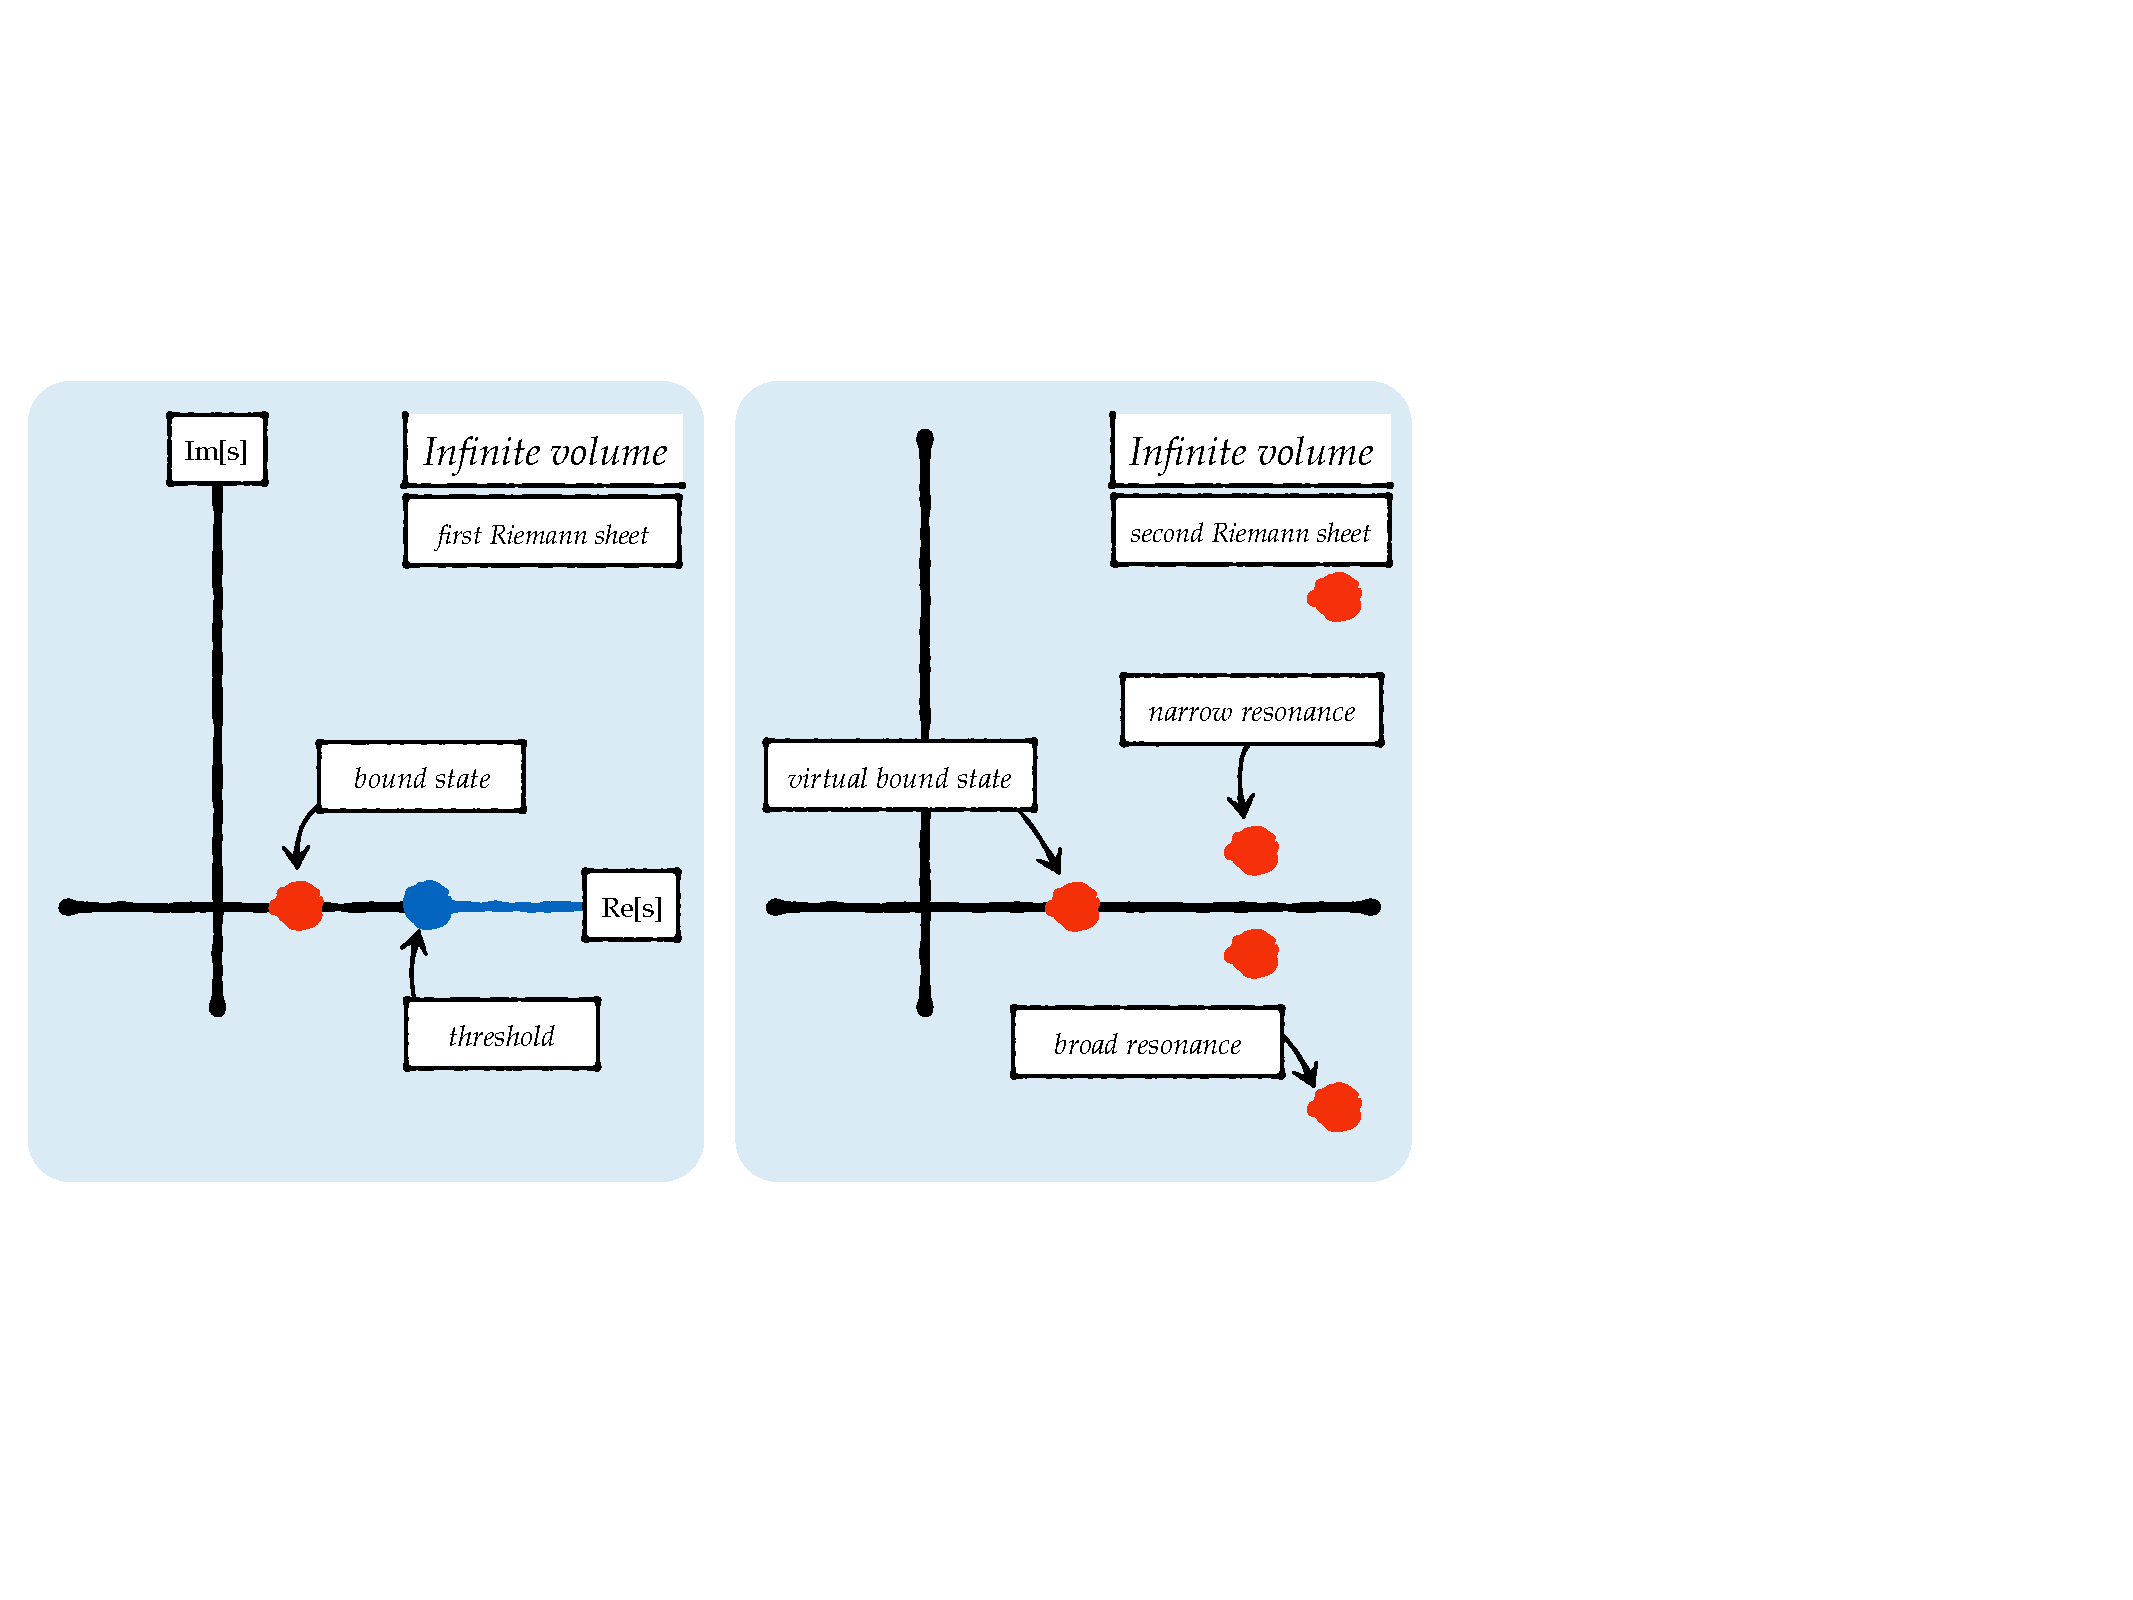
\includegraphics[scale=0.29]{infinite_volume_spec}
\label{fig:IV_spec}}
\hspace{1cm} 
\subfigure[]{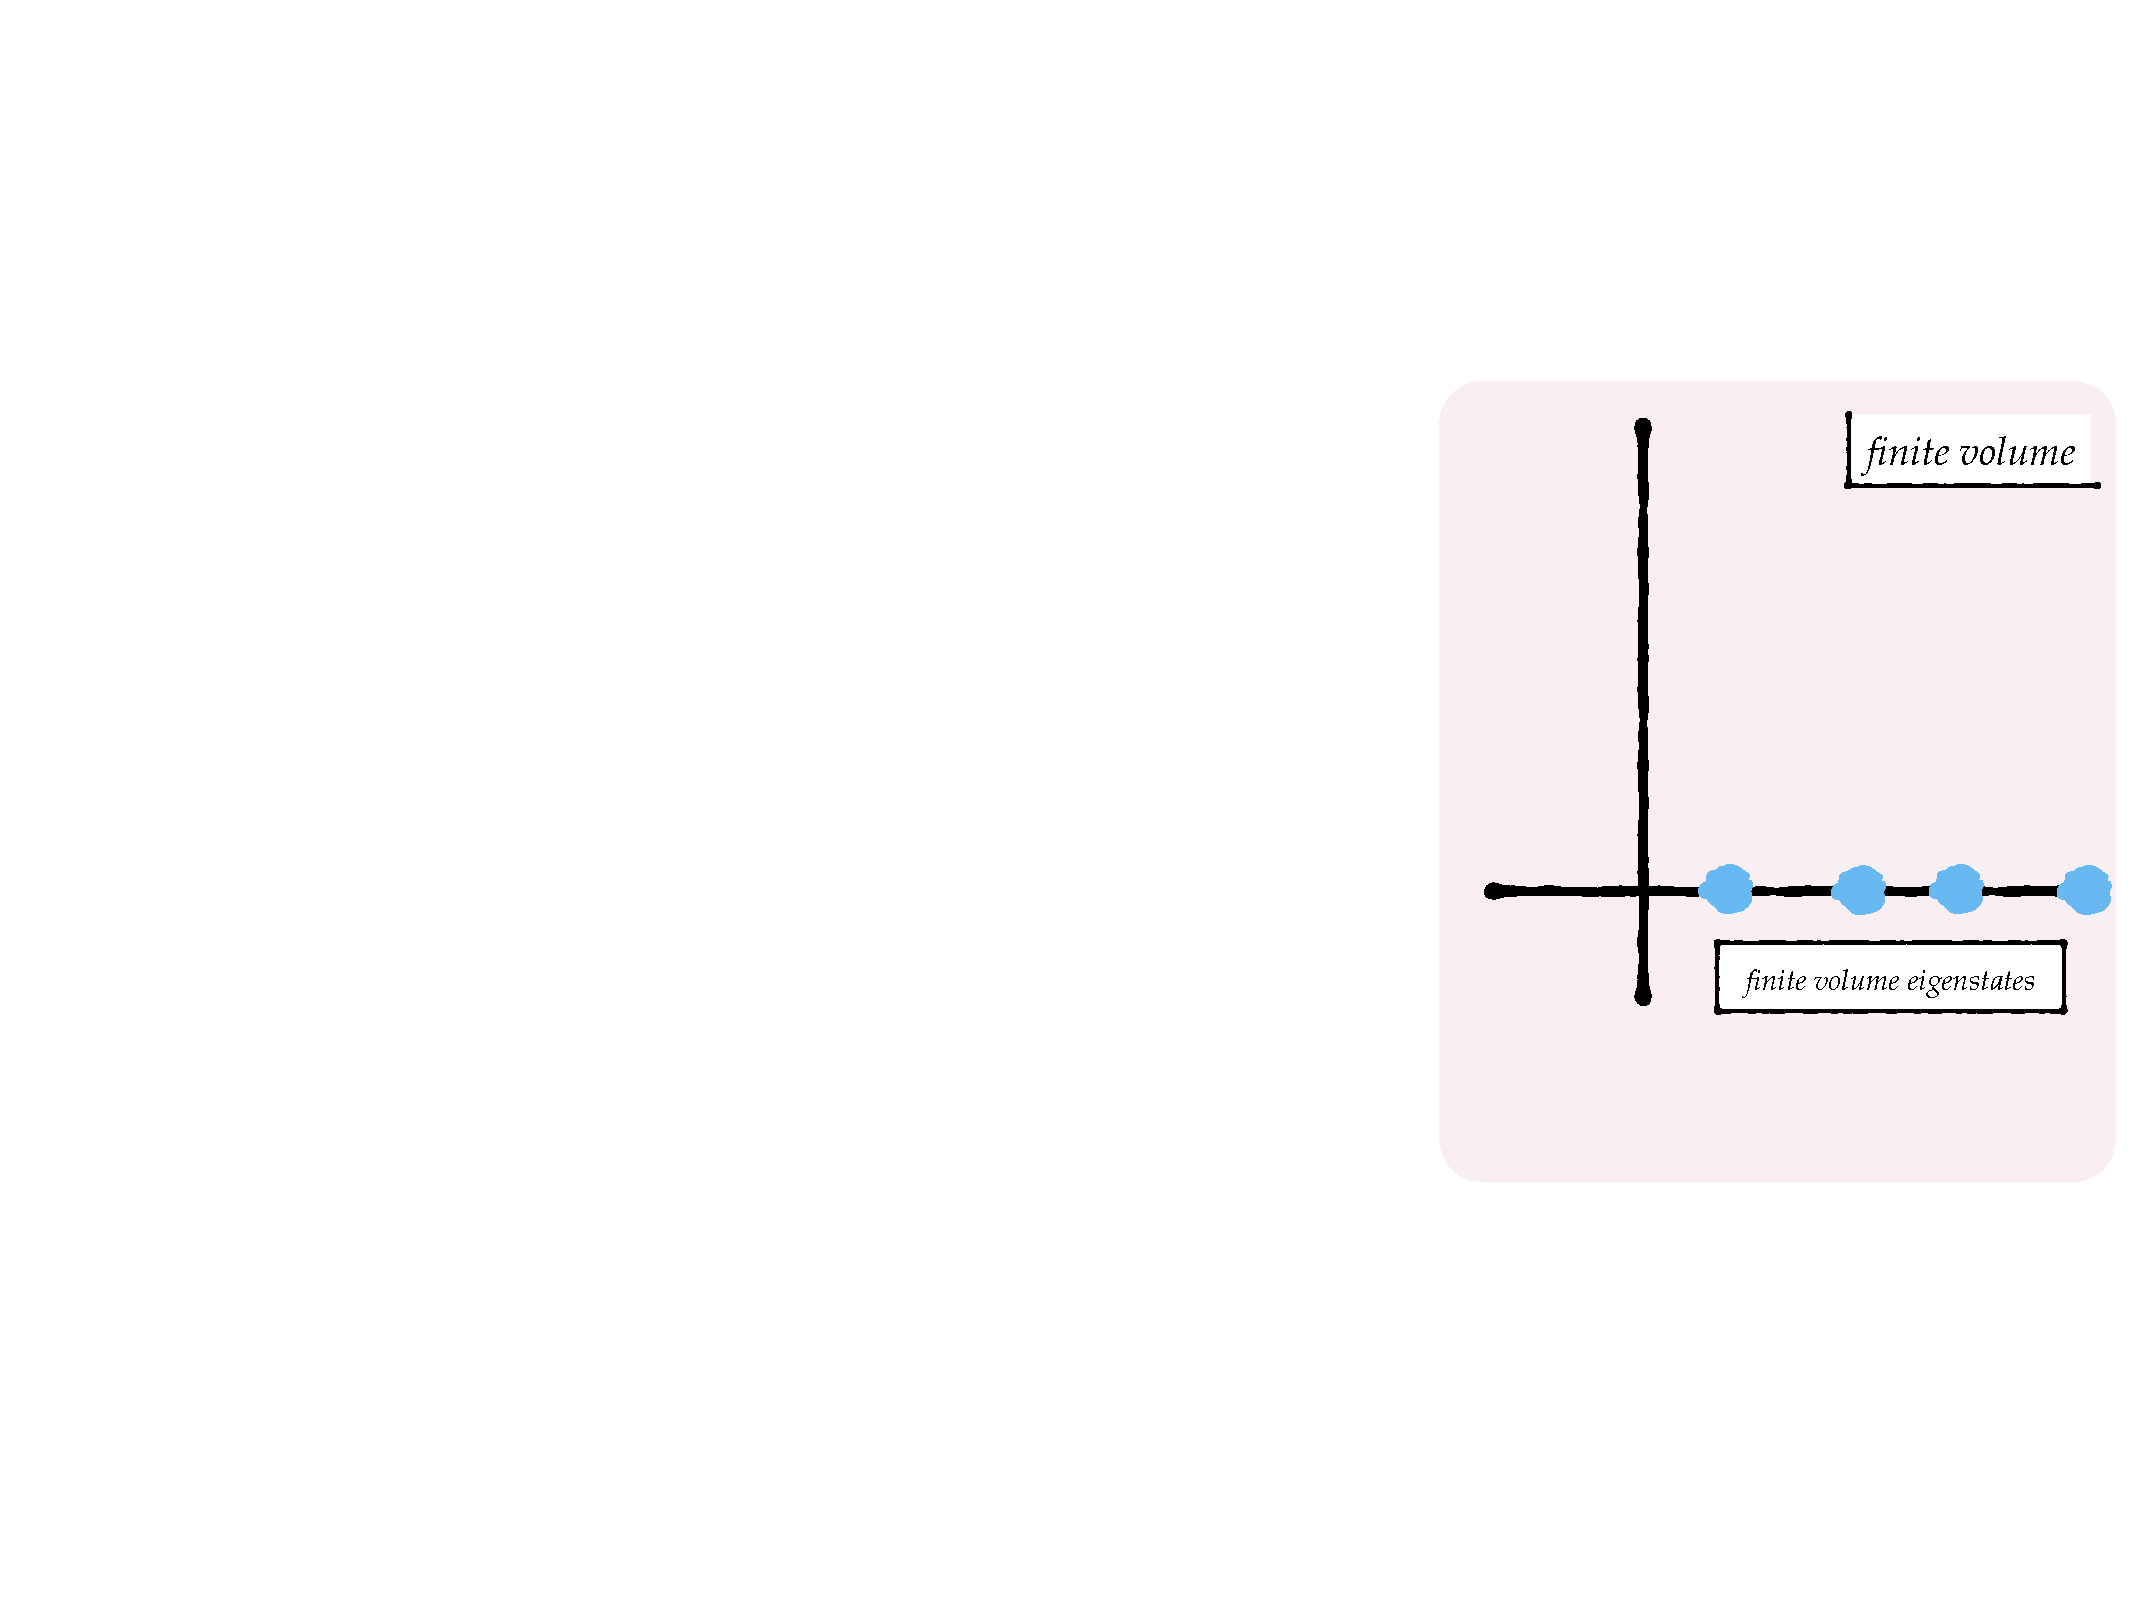
\includegraphics[scale=0.29]{finite_volume_spec}
\label{fig:FV_spec}}
% figure caption is below the figure
\caption{(a) Shown is a cartoon depiction of the analytic structure of the infinite-volume scattering amplitude. This is compared with the (b) finite-volume spectrum. Details are discussed in the text. [This figures were first shown in Ref.~\cite{Briceno:2016cxt}.]
}
\label{fig:toy_spec} 
\end{figure}
%%%%%%%%%%%%%%%%
%%%%%%%%%%%%%%%%


A more rigorous definition of these states can be obtained from the analytic structure of the scattering amplitude of the channel that contains the same quantum numbers of the state of interest. In particular, all composite particles can be understood as poles in the scattering amplitude, $\mathcal{M}$. It is convenient to begin by reviewing the definition of the scattering amplitude for systems composed of two scalar bosons. Furthermore, we restrict our immediate attention to energies where only one channel is kinematically open. If we label the full scattering amplitude as $\mathcal{M}$, we can write down the partial wave projection of this as 
\begin{eqnarray}
\mathcal{M}(P)=\sum_{\ell,m_\ell}\sum_{\ell',m_\ell'}\,
Y^*_{\ell m_\ell}(\hat {\mathbf q}^*) \,
\mathcal{M}_{\ell,m_\ell;\ell',m_\ell'}(E^*)\,
Y_{\ell' m_\ell'}(\hat  {\mathbf q}^*),
\end{eqnarray}
where $\ell$ and $m_\ell$ label the angular momentum and its azimuthal component. $E^*$ and $\hat {\mathbf q}^*$ are the center of mass (c.m.) energy and momentum. These are related to the four momentum of the system in the standard way, 
\begin{eqnarray}
s=\sqrt{P^2}=\sqrt{E^2-\mathbf{P}^2}=E^{*}=\sqrt{m_1^2+{ q}^{*2}}+\sqrt{m_1^2+{ q}^{*2}},
\end{eqnarray}
where we have introduced the Mandelstam variable $s$. Using this expression, we can solve for $q^*$,
\begin{eqnarray}
q^*=\frac{1}{2}\sqrt{E^{*2}-2\,(m_1^2+m_2^2)+\frac{(m_1^2-m_2^2)^2}{E^{*2}}}
\end{eqnarray}
Conservation of angular momentum requires the scattering amplitude to be diagonal in $\ell$. Azimuthal symmetry tells us that all $m_\ell$ components of the scattering amplitude are identical. In summary, the scattering amplitude satisfies the following expression,
\begin{eqnarray}
\mathcal{M}_{\ell,m_\ell;\ell',m_\ell'}
=\delta_{\ell\ell'}\,\delta_{m_\ell m_\ell'}\,\mathcal M_{\ell}.
\end{eqnarray}
Furthermore, unitarity allows us to write $\mathcal M_{\ell}$ in terms of kinematic factors and a single dynamical function namely the scattering phase shift, $\delta_{\ell}$,~\cite{Kim:2005gf}
\begin{eqnarray}
\mathcal M_{\ell}=\frac{8\pi E^*}{\xi}\frac{1}{q^*\cot\delta_{\ell}-iq^*} \,,
\label{eq:scatamp}
\end{eqnarray}
where $\xi$ is a symmetry factor, equal to $1/2$ if the particles are identical and $1$ otherwise. 

Near threshold, one can show that $q^*\cot\delta_{\ell}$ is a polynomial in $s$. This is commonly known as the \emph{effective range expansion}. On the other hand, the imaginary term leads to a square root in $s$, which in turn introduces a branch point at threshold. The presence of a branch cut is closely tied to the fact that there is a continuum of states. This branch point forces us to consider the Riemann sheet structure of the scattering amplitude. For the simple example considered, there are only two sheets present. By aligning the branch cut starting at threshold and moving to positive infinity [as depicted in Fig.~\ref{fig:IV_spec}], the two sheets can be defined by the sign of the imaginary component of $q^*$. The first (or physical) Riemann sheet satisfies $\sign[{\rm Im} (q^*)]\geq0$, while the second (or unphysical) sheet satisfies $\sign[{\rm Im} (q^*)]<0$. 

Although the sheet structure of the scattering amplitude might seem as a \emph{nuance}, this has profound physical consequences. To understand these, we also need to recognize that the scattering amplitude can have poles. From Eq.~\ref{eq:scatamp}, it is clear these poles must satisfy $q^*\cot\delta_{\ell}=iq^*$. Depending where the poles are present in the complex plane, it leads to the three scenarios of composite particles discussed above. For clarity, we list these cases
\begin{itemize}
  \item Bound state: real pole on the physical sheet below threshold.
  \item Virtual bound state: real pole on the unphysical sheet below threshold.
  \item Resonance: complex pole on the unphysical sheet above threshold. 
\end{itemize}
A pictorial representation of these are shown in Fig.~\ref{fig:IV_spec}. For a single open channel, each resonance pole emerges with its complex conjugate partner. {\raul[ Maybe cite Pennington for counterexamples]}. The fact that there are no poles with imaginary components in the first Riemann sheet is a consequence of causality.
%%%%%%FOOTNOTE%%%%%%
\footnote{We point the reader to Ref.~\cite{Gribov:1186219} for a proof.}
%%%%%%FOOTNOTE%%%%%%	





 The mass ($m_R$) and decay width ($\Gamma_R$) of the resonance can be directly accessed from the real and imaginary components of the pole location, $s_{pole}$, $m_R\equiv {\rm Re}({E_{pole}})$, $\Gamma_R\equiv -2~{\rm Im}({E_{pole}})$. Since the poles associated with real and virtual bound states are purely real, their decay width are also zero -- as one would expect. The reason why it is important to recognize that resonances are just one of the three types of composite states is because, depending on the values of the parameters of QCD, namely the quark masses, one state can transition from being bound to being a resonance or a virtual bound state. Perhaps the most famous example of this is the $\rho$ meson, which for quark masses corresponding to $m_\pi \gtrsim 400$~MeV is a physical bound states but for lighter quark masses it is a resonance, as is depicted in Fig.~\ref{fig:rho_mpi_0}. 
 
 
Placing QCD in a finite volume leads to a discreet, real spectrum [as depicted in Fig.~\ref{fig:FV_spec}] and the absence of a branch cut. Having a single sheet, all poles of the correlation function lie on the physical sheet, making the direct determination of resonance poles from lattice QCD impossible. A reliably way to circumvent this is to extract from the finite-volume spectrum the infinite-volume scattering amplitude. Having obtained this for a large kinematic regimue, one can then study its analytic structure to deduce its poles in the complex plane. Given that the finite-volume spectrum is constrained to be real, one should only expect a direct constraint to scattering amplitudes for real values of the energy of the system. One must rely on analytic constraints of scattering amplitude to deduce information about resonances. This, of course, closely mirrors the experimental situation. {\raul [maybe cite Ref.~\cite{Pelaez:2015qba} and the $\sigma$ as a indicative example of where this is most important]}. In the subsequent sections we will mainly focus on the first goal, which is to understand how scattering amplitudes can be obtained from the lattice QCD spectrum. 





%%%%%%%%%%%%%%%%
%%%%%%%%%%%%%%%%
\begin{figure}[t]
\centering
{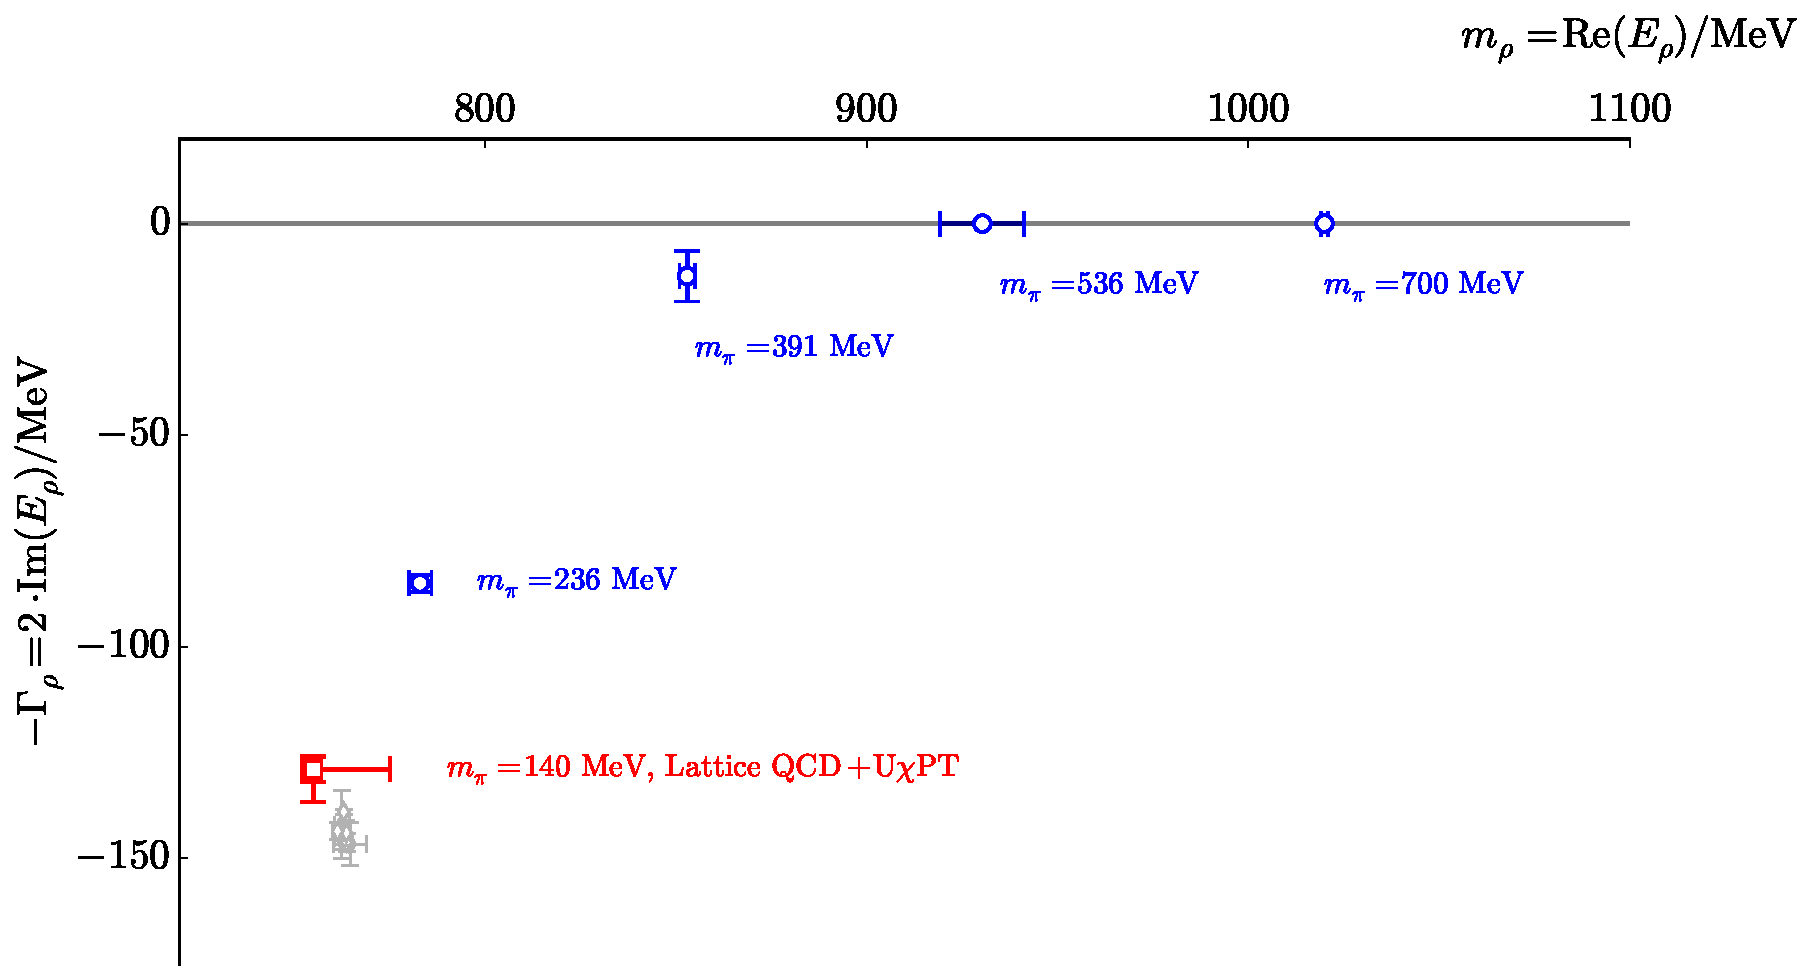
\includegraphics[scale=0.3]{rho_mpi_0}}
\caption{ Shown is the quark-mass dependence of the $\rho$ pole. Shown in blue are with previous lattice calculations performed using unphysically heavy quark masses where the $\rho$ is stable~\cite{Lin:2008pr} as well as unstable~\cite{Dudek:2012xn, Wilson:2015dqa}. The red square shows the chiral extrapolation presented in Ref.~\cite{Bolton:2015psa} of the results obtained in Ref.~\cite{Wilson:2015dqa}, and it is compared with solutions to the Roy equation~\cite{Roy:1971tc} constrained from experimental data [grey diamonds]~\cite{Masjuan:2014psa, Ananthanarayan:2000ht, Colangelo:2001df, Zhou:2004ms, GarciaMartin:2011jx, Masjuan:2013jha}.
.}
\label{fig:rho_mpi_0} 
\end{figure}
%%%%%%%%%%%%%%%%
%%%%%%%%%%%%%%%%
%%%%%%%%%%%%%%%%

\subsection{Diagrammatic definition of the scattering amplitudes}
For the derivations that follow, it is convenient to bare in mind a diagrammatic definition of scattering amplitudes. Before discussing this, we must clarify one key point. QCD is a theory whose fundamental degrees of freedom are quark and gluons. Being that these are confined, asymptotic states can only be composed of hadrons. Therefore, although we have QCD in mind through this work, the Feynman diagrams we will be discussing are those of the asymptotic states of QCD, namely hadrons. One could always envision that QCD can be mapped onto an all-encompassing low-energy effective field theory (EFT), which dictates all of the dynamics of hadrons. For most intense and purposes, we will not need to make a direct reference to this EFT or even need to write down the corresponding Lagrangian density. All we will need to do is postulate that such theory and Lagrangian exists and it satisfies all symmetries and constraints put in place by QCD.

Now we may proceed to define scattering amplitudes of hadrons in terms of Feynman diagrams. Of course, this is in general very straightforward to do. If we are interested in a process with $n$ incoming and $n'$ outgoing hadrons, the corresponding scattering amplitude, $\mathcal{M}(n\to n')$, is defined as
\theoremstyle{definition}
\begin{definition}
{$\mathcal{M}(n\to n')$} = the sum over all diagrams with $n$ incoming and $n'$ outgoing legs that have been amputated and put on-shell.
\end{definition} 
\noindent
The challenge if, of course to sum diagrams that satisfy this criterium to all order in the perturbative expansion, whatever that may be. Lattice QCD being non-perturbative in the strong force, all diagrams are included. 


\subsection{Multichannel systems with arbitrary spin}
One can readily generalize the discussion above to energies where more than one channel is kinematically open. For such a scenario, it is convenient to introduce an index $``a"$ that runs over all open channels. The scattering amplitude becomes a matrix in this space. The component $\mathcal M_{ab}$ denotes the scattering amplitude with incoming an incoming $``a"$ state and outgoing $``b"$ state. Granted time-reversal symmetry the scattering amplitude must be symmetric, meaning $\mathcal M_{ba}=\mathcal M_{ab}$. Furthermore, just like in the single-channel case, unitarity places a strong constraint on the form that the scattering amplitude can take. This is most evident when we write the scattering amplitude in terms of S-matrix. 

To do this we introduce a diagonal phase-space matrix,
\begin{eqnarray}
\mathbb{P}={\rm{diag}}(\sqrt{\xi_1q^{*}_1},\sqrt{\xi_2q^{*}_2},\ldots,\sqrt{\xi_Nq^{*}_N})/\sqrt{4\pi E^*},
\end{eqnarray}
where $\xi_a$ and $q^{*}_a$ are the symmetry factor and relative momentum for the $ath$ channel. This leads to the following relation between $\mathcal M$ and S~\cite{Hansen:2012tf}
%
\begin{eqnarray}
i\mathcal{M}=\mathbb{P}^{-1}~{(S-1)}~\mathbb{P}^{-1}.\label{eq:Smatrix}
\end{eqnarray}
By definition, the S matrix must satify $S^\dag S=1$. For a single channel, the S matrix is scalar and equal to $e^{i2\delta_\ell}$. It is a simple excercize to show that using this expression for the S matrix in Eq.~\ref{eq:Smatrix} leads to Eq.~\ref{eq:scatamp}. 


\begin{eqnarray}
\mathcal{M}^{-1}=\mathcal{K}^{-1}-i\,\mathbb{P}^{2}/2.\label{eq:Kmatrix}
\end{eqnarray}


%%%%%%%%%%%%%%%%%%%%%%%%%%%%%%%%%%%%%%%%%%%
\begin{figure*}[t]
\begin{center}
\subfigure[]{
\label{fig:scat_ampa}
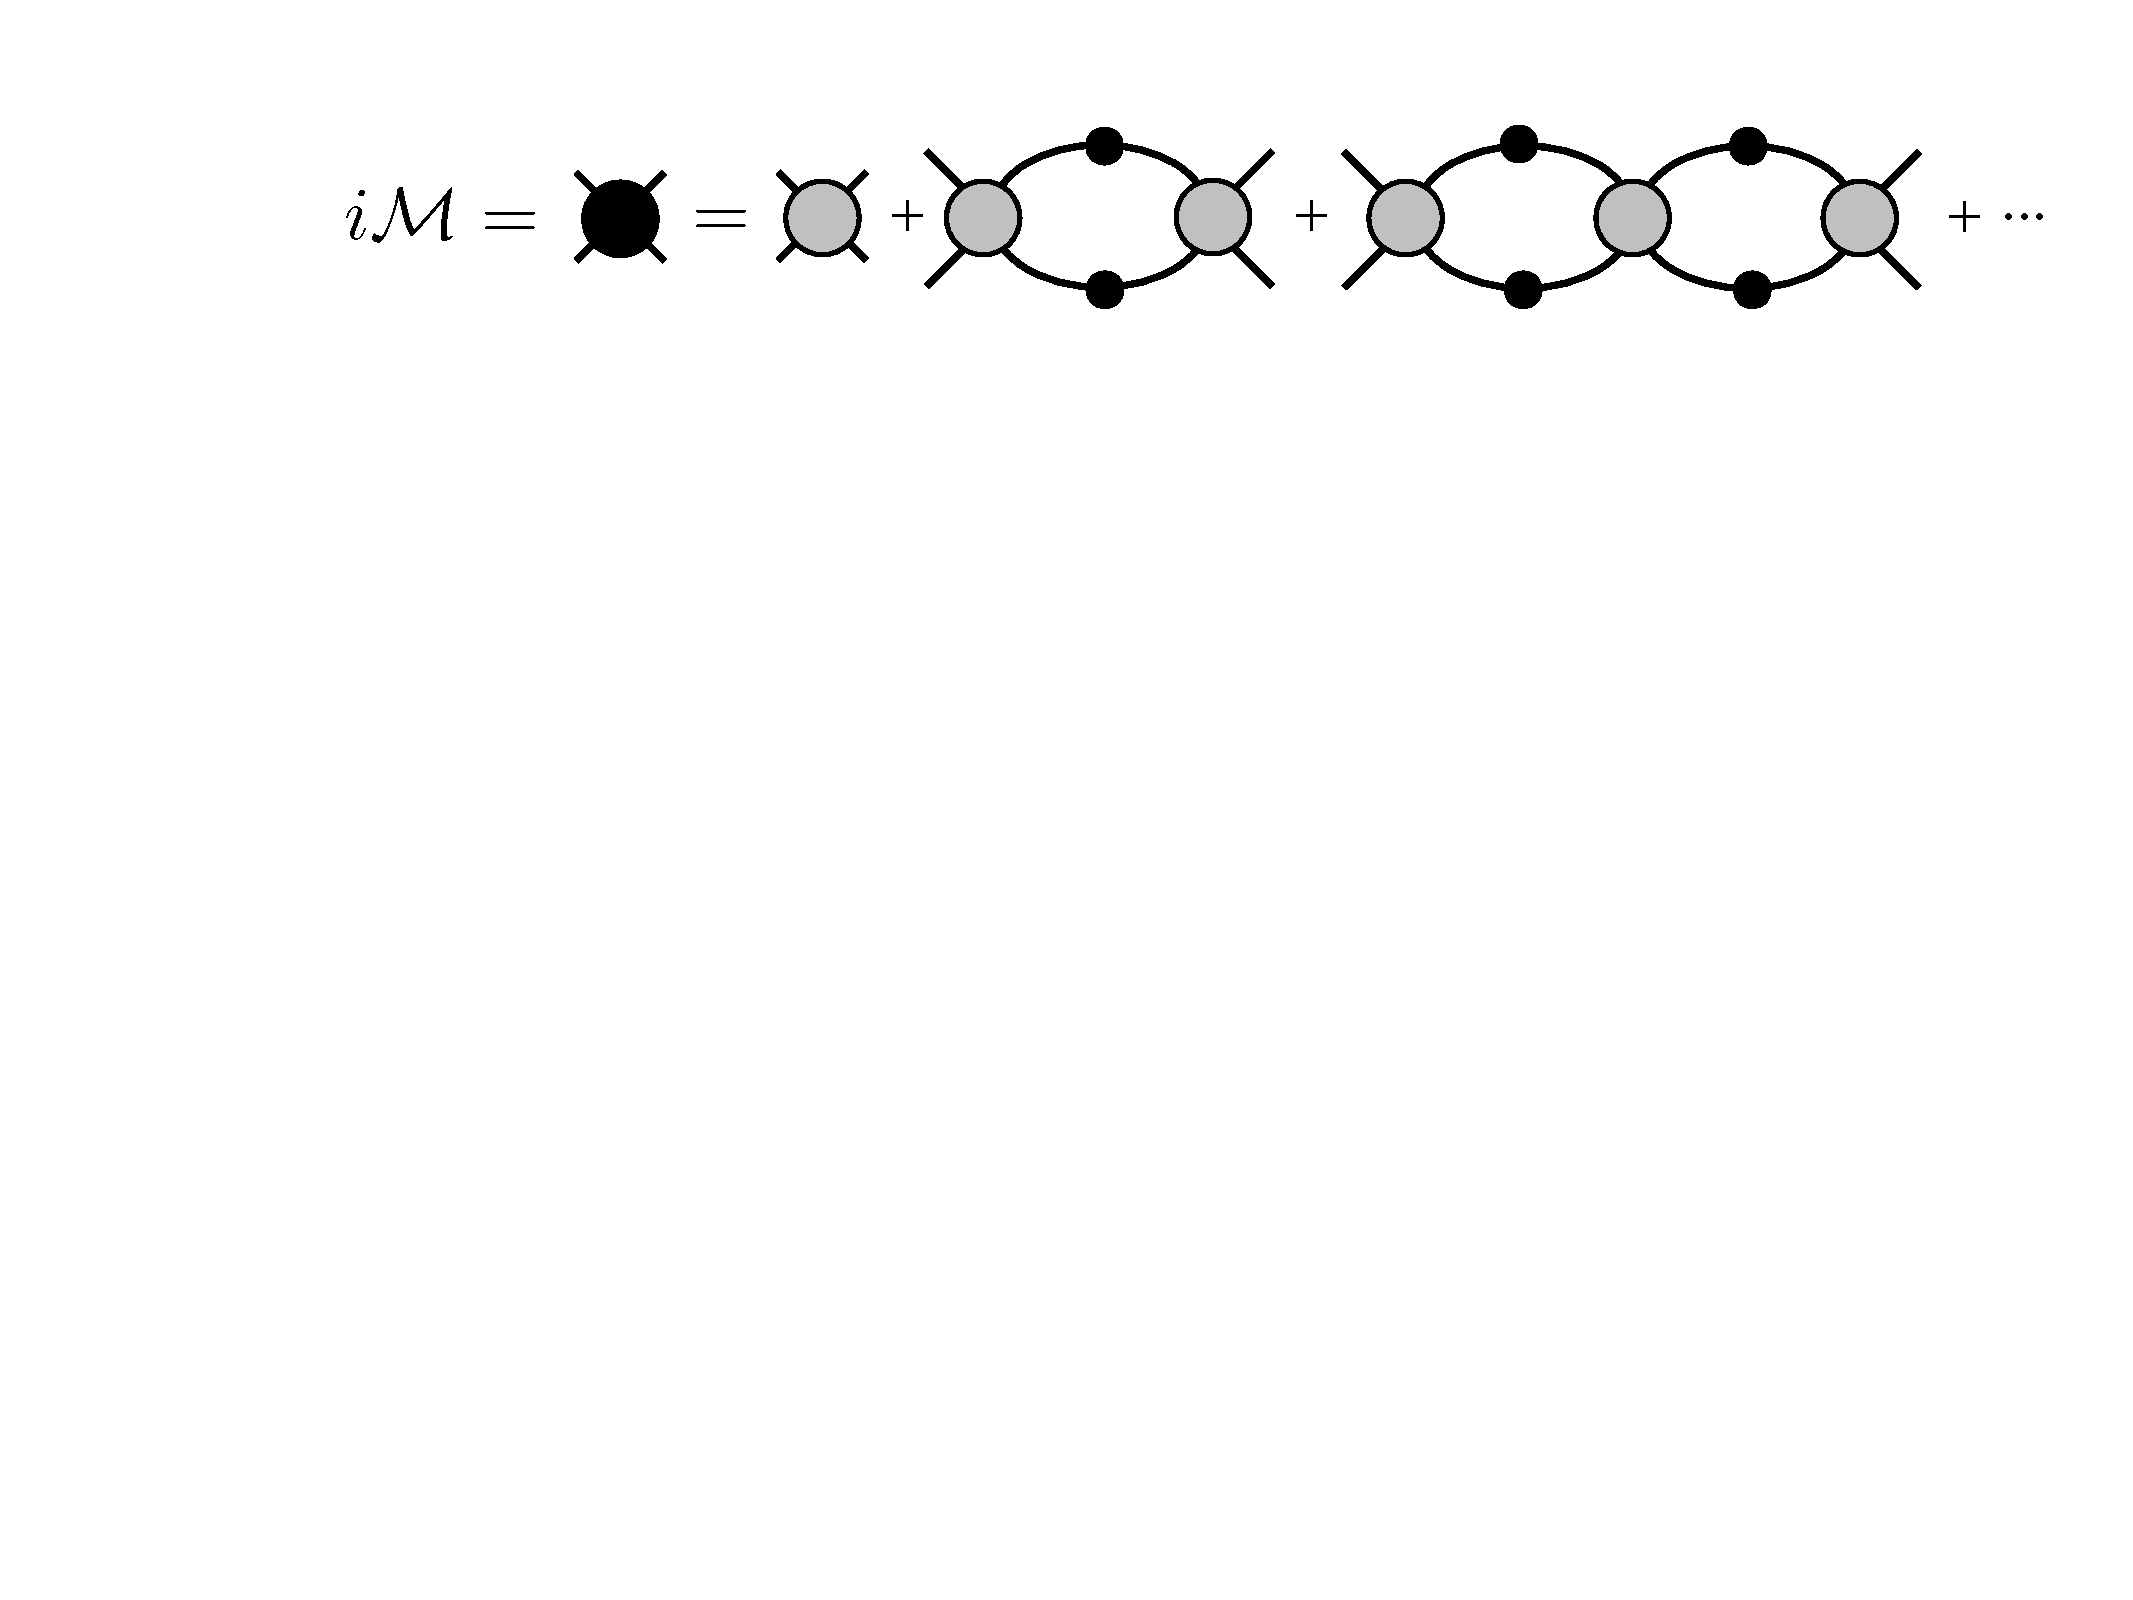
\includegraphics[scale=0.4]{scat_amp}}\\
\subfigure[]{
\label{fig:kernel}
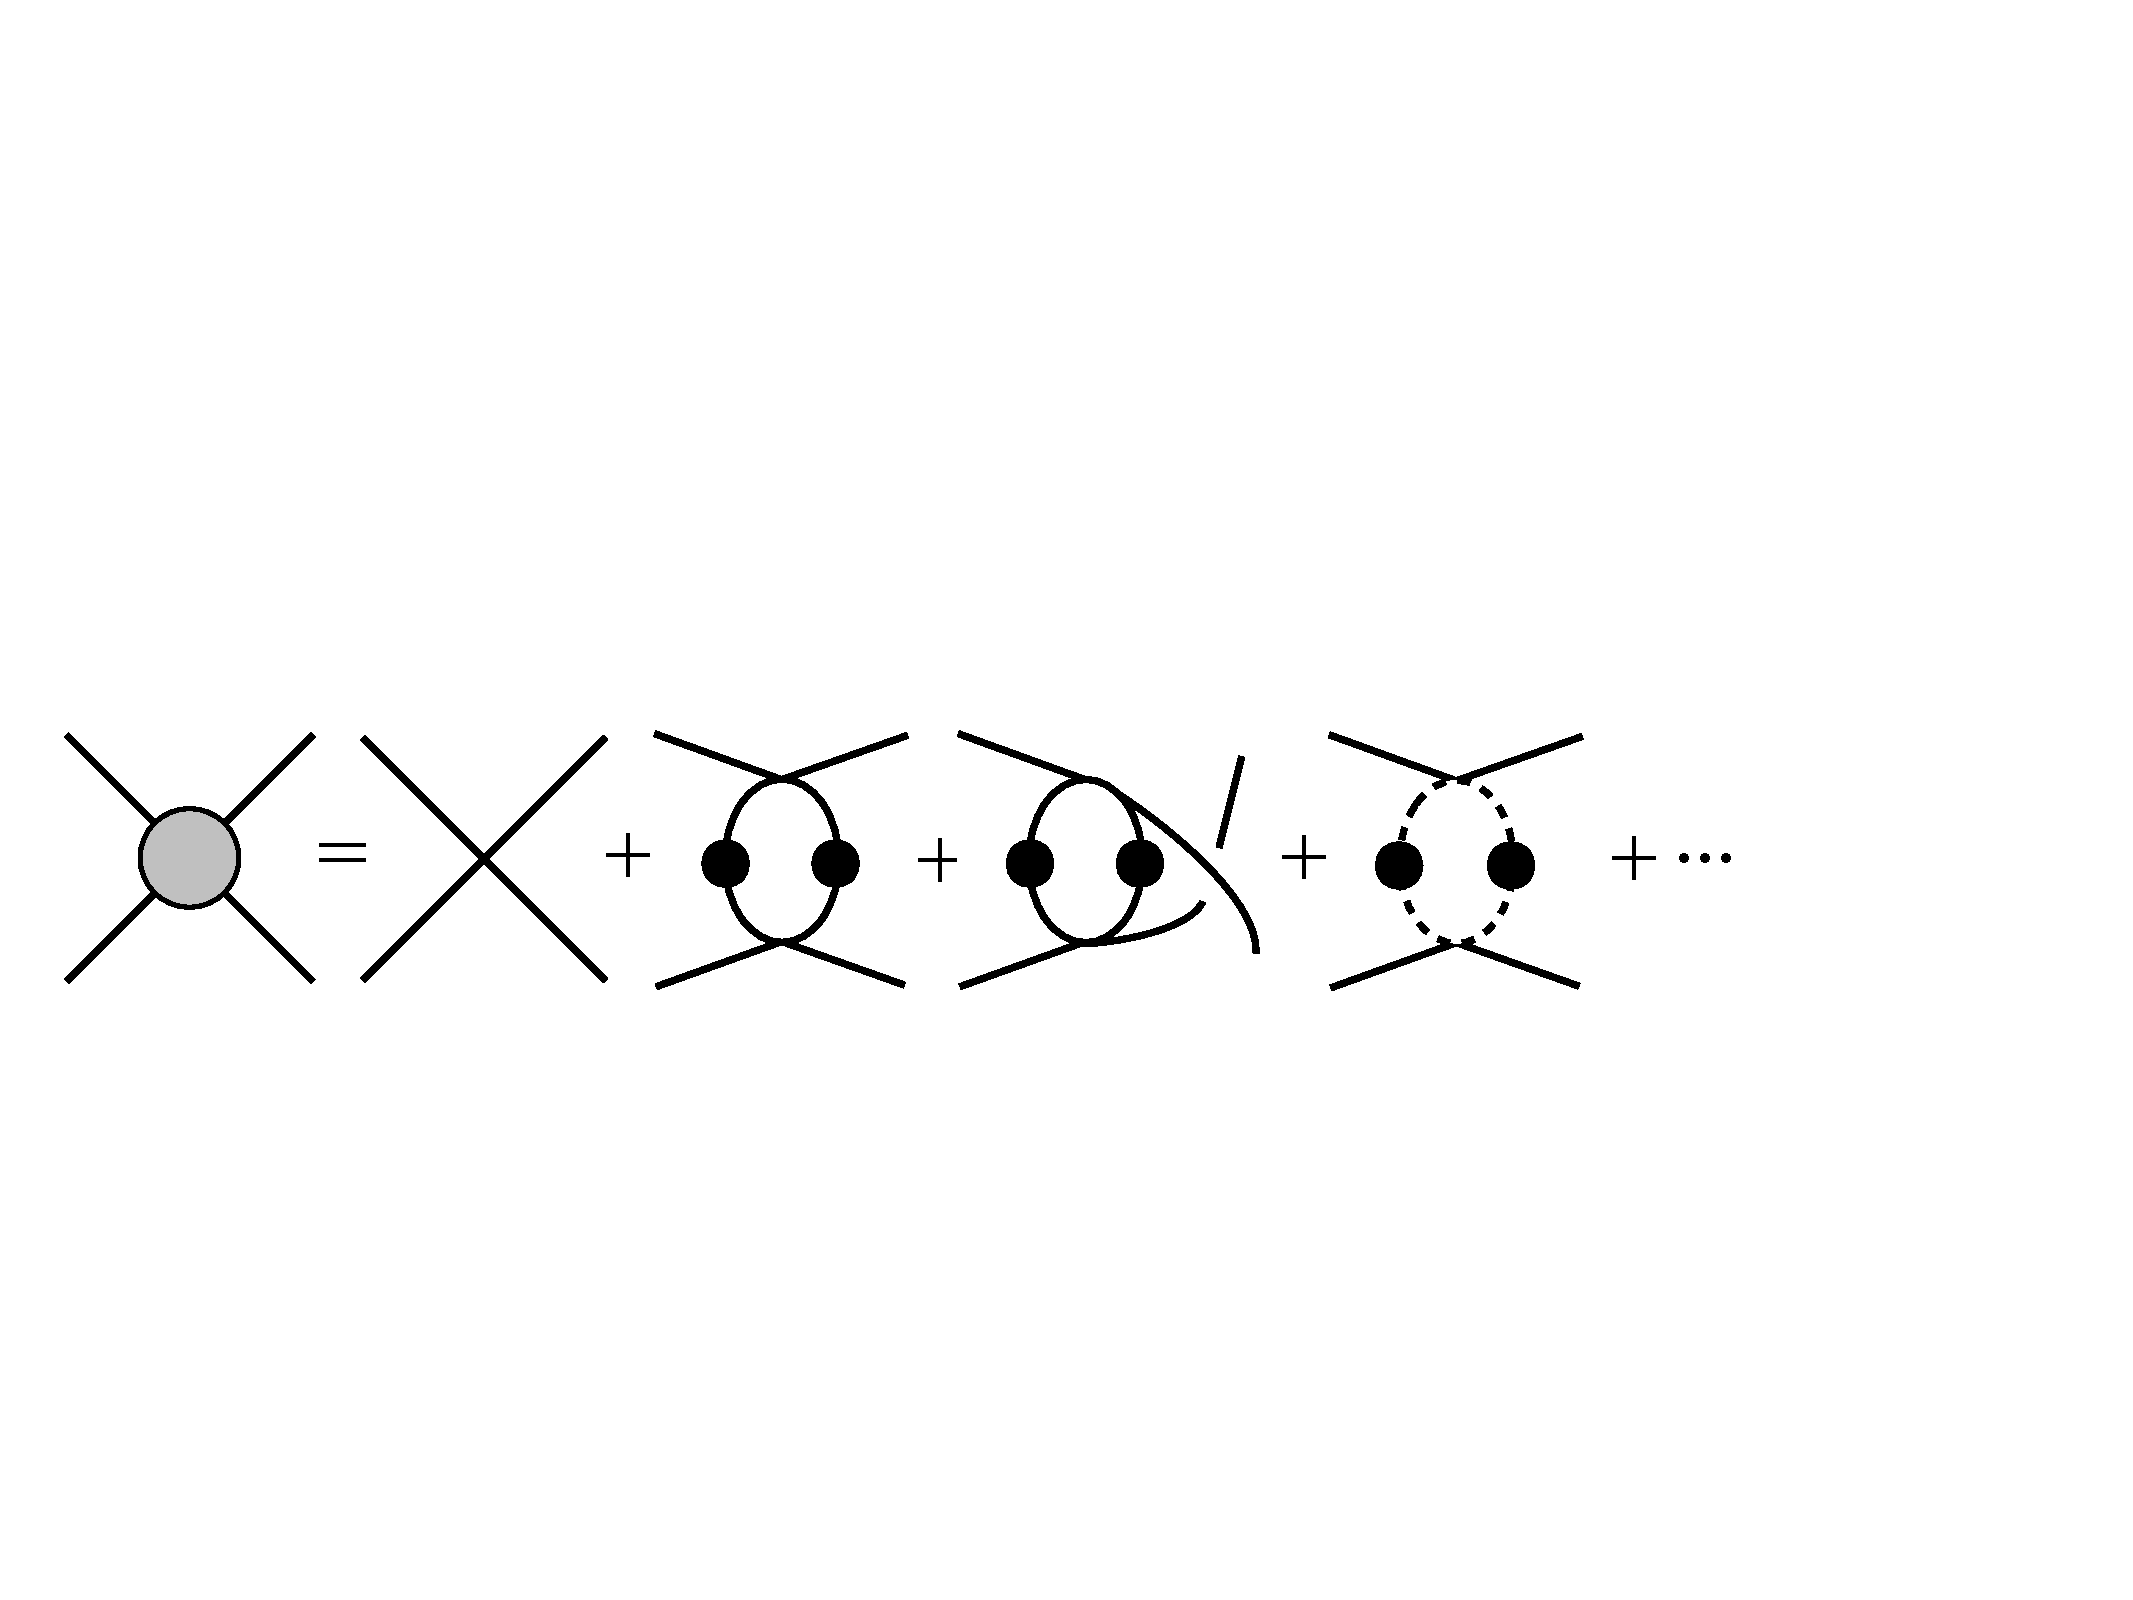
\includegraphics[scale=0.2]{kernel}}
\subfigure[]{
\label{fig:1bodyprop}
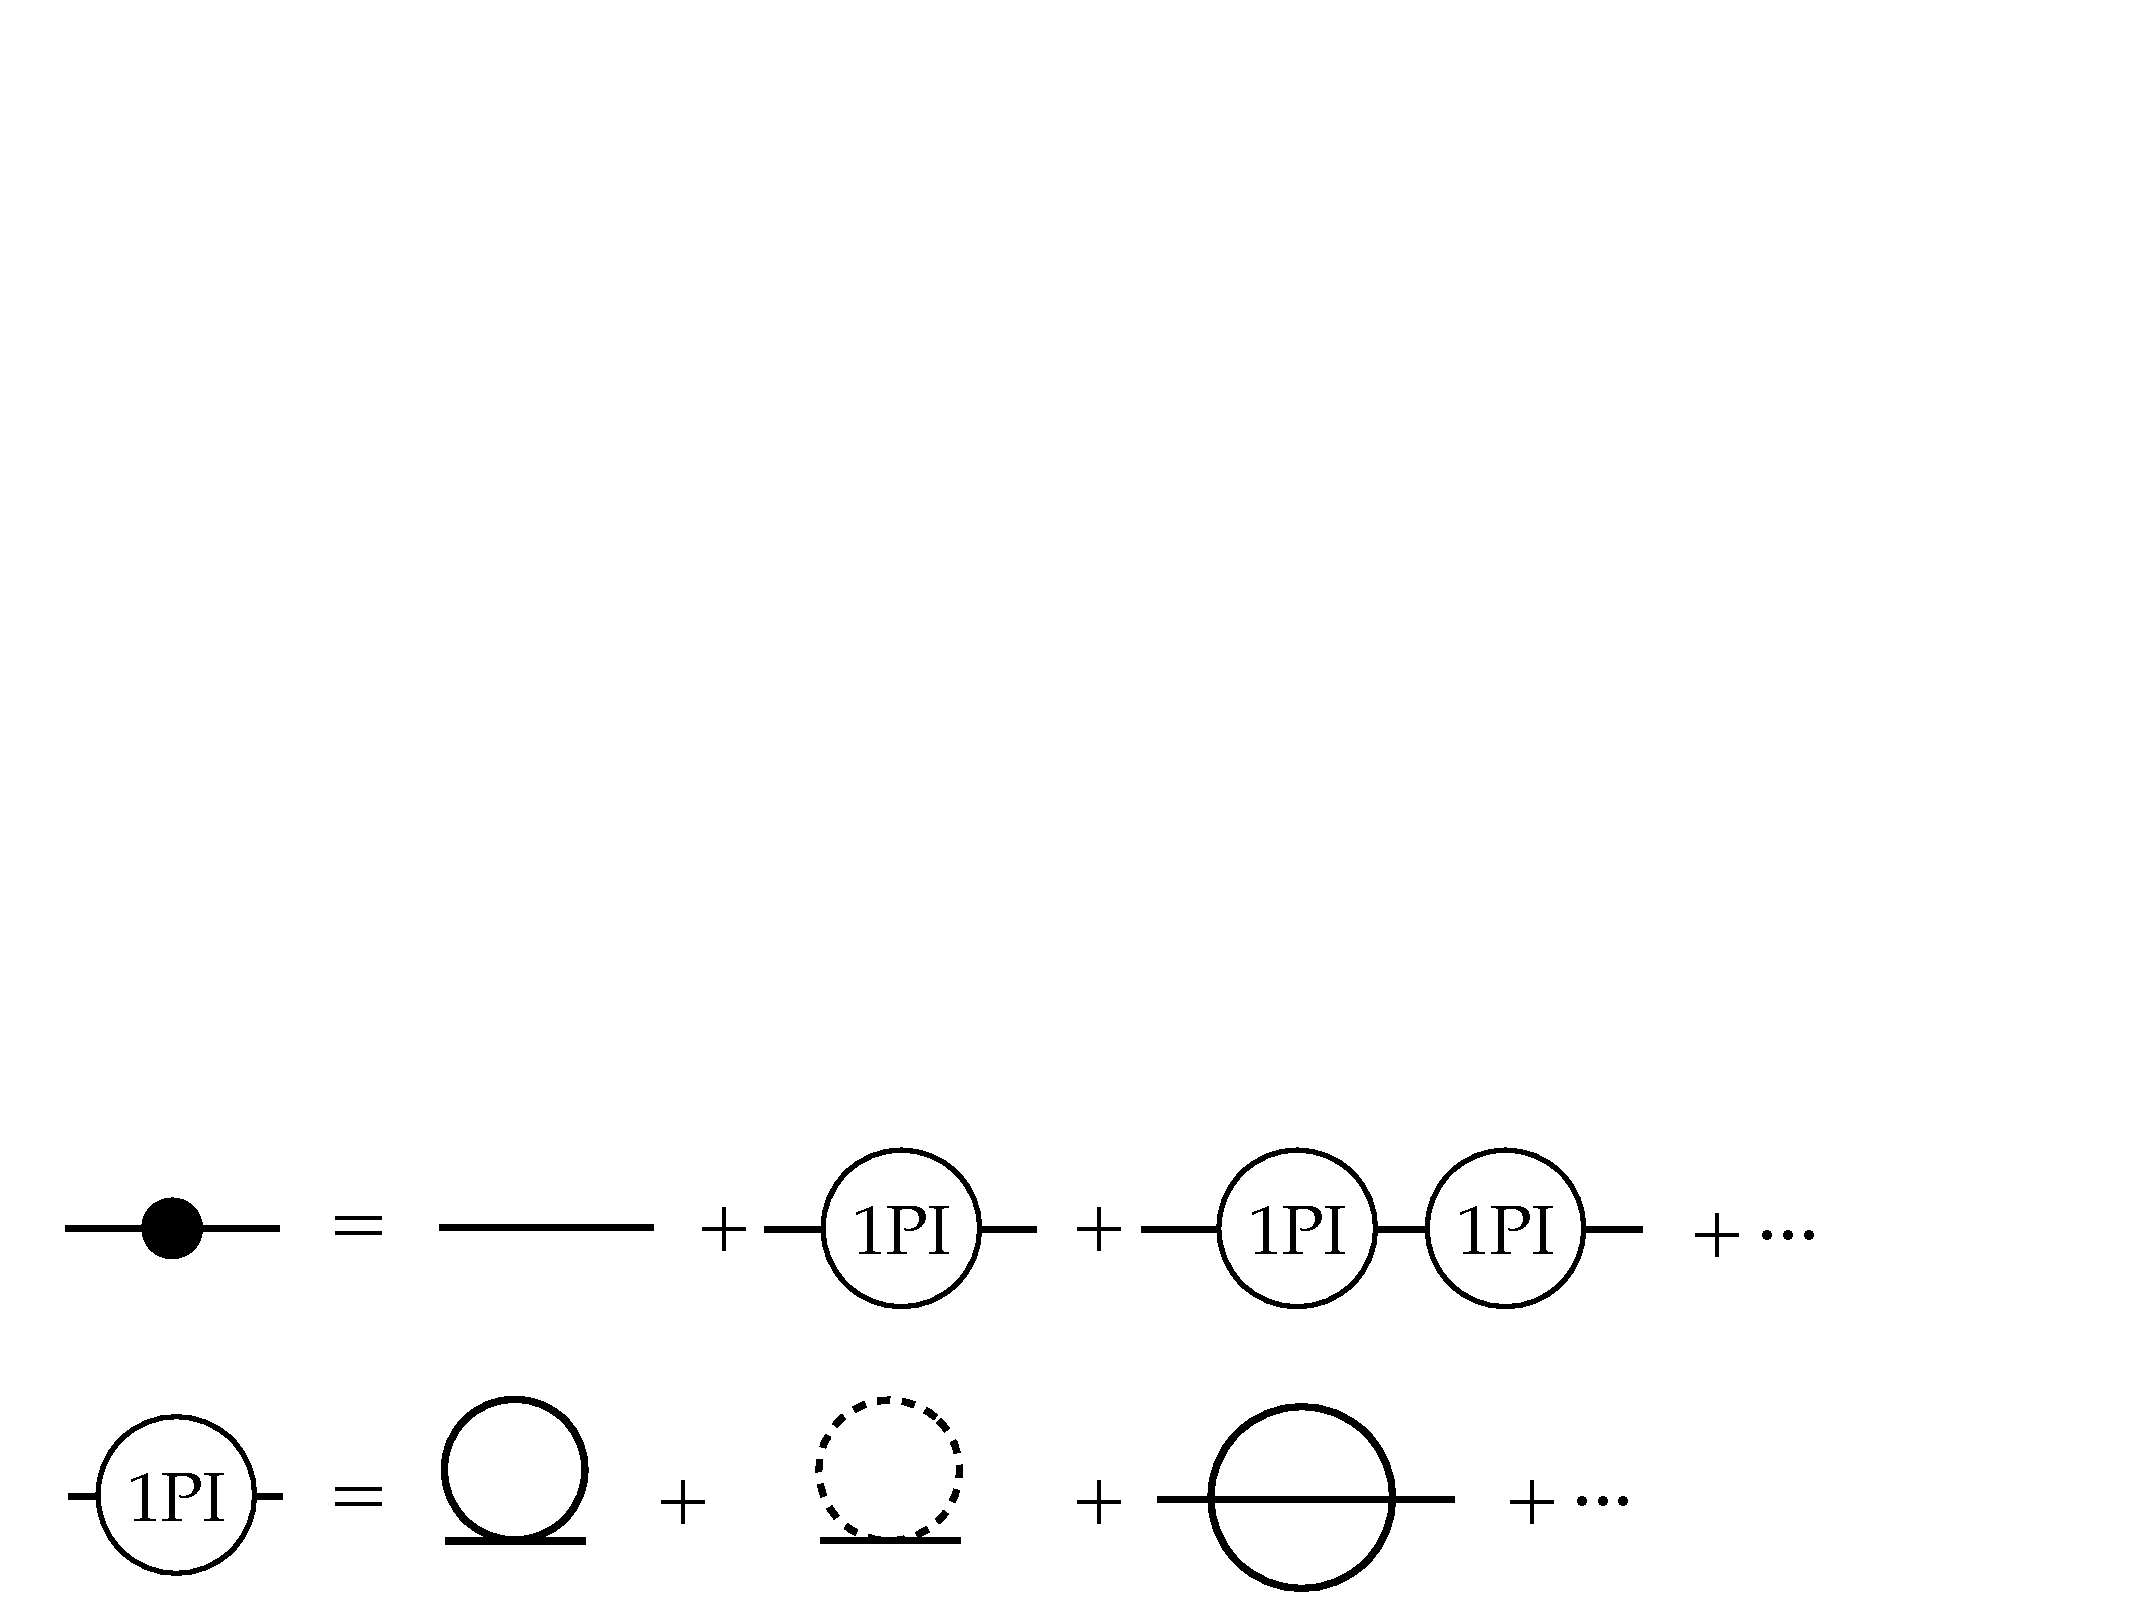
\includegraphics[scale=0.2]{1bodyprop}}

\caption{ (a) The scattering amplitude, $\mathcal M$, is defined as the sum over all on-shell, amputated four-point diagrams. This can be written in terms of the Bethe-Salpeter kernel (b) and the fully-dressed single body propagator (c). The Bethe-Salpeter kernel is given by the sum of all amputated four-point diagrams which are two-particle irreducible in the channel carrying the total energy and momentum. This quantity is useful in the present context because, for the kinematics we consider, the difference between its finite- and infinite-volume form is exponentially suppressed in the box size. The same is true for the fully dressed propagator.}\label{fig:scat_amp}
\end{center}
\end{figure*}
%%%%%%%%%%%%%%%%%%%%%%%%%%%%%%%%%%%%%%%%%%%

\section{Resonance form factors from lattice QCD \label{Sec:formfactors}}

As discussed in the previous section, the field has witnessed an impressive amount of progress in the ability to determine masses and widths of hadronic resonance. In particular, a general quantization condition for two-particle systems in a finite volume has been derived, {\raul see Eq.~{??}}, and it has been successfully implemented in various numerical calculations. Furthermore, although there is no present universal formalism in place suitable for the analysis of energies above multi-particle thresholds, we have reviewed the first steps towards finding such an equation. 

Ultimately, the determination of masses and width serve only as the first steps towards a robust determination of hadronic resonances. Once we have determined their pole positions, we can then begin to ask question regarding their inner structure and transitions mediated by the electroweak sector of the standard model. Due to the altered analytic structure of QCD when placed in a finite volume, we once again must rely on formalism to map the quantity directly obtained the correlation function evaluated via lattice QCD and the desired infinite-volume observables. In this section we review recent progress toward this aim.

To this day, the vas majority of lattice QCD treated QCD non-perturbatively, while electroweak quantities are obtained only at leading order in the electroweak interaction. This allows one to access this quantities  using either the insertion of external currents or placing the system in the presence of an external background/auxiliary field. To this say, the background field method has not been used to study matrix elements of scattering/resonating states, so we pay a closer attention to the direct evaluation of matrix elements of external currents. We dedicate Sects.~\ref{sec:LL_formalism}, \ref{sec:2body_mat} and \ref{sec:perturbative_results} to review the theoretical developments needed to analyze finite volume matrix elements involving states that coupled to two particles or more. In Sect.~\ref{sec:background_field} we discuss similar developments in the use of background field methods.  

There has been some progress towards the incorporation of non-perturbative QED in lattice QCD calculation~{\raul [cite] \cite{Endres:2015gda}}. Such calculations are still in their developmental stages and to this day there has been no lattice scattering processes or resonance using lattice QCD+QED. Nevertheless there was been recent theoretical development showing that QED corrections to elastic scattering amplitudes of two-body systems can be studied via lattice QCD+QED calculation~\cite{Beane:2014qha}. which we review in Sect.~\ref{sec:trans_amps}.

Before discussing the necessary finite-volume formalism, we first the physical quantities we are after. As thoroughly discussed in the previous section, from the finite-volume spectrum one can access the infinite-volume scattering amplitude. It is not hard to imagine that the quantity that emerges from evaluation of matrix elements of electroweak is closely related to the scattering amplitude with an external leg attributed to the external field ({\raul see Fig.~X}). Given that the electroweak sector is only treated to leading order, the resulting amplitude is exact/non-perturbative in QCD but only suitable up to leading-order in the perturbative expansion of the electroweak sector. In this work, we will adopt the nomenclature used in Refs.~\cite{Briceno:2014uqa, Briceno:2015csa, Briceno:2015tza} and refer to such amplitudes that are immediately accessible from lattice QCD as \emph{transition amplitudes}. These will be more carefully defined for various processes in Sect.~\ref{sec:trans_amps}. 




%%%%%%%%%%%%%%%%
%%%%%%%%%%%%%%%%
\begin{figure}[t]
\centering
\subfigure[]{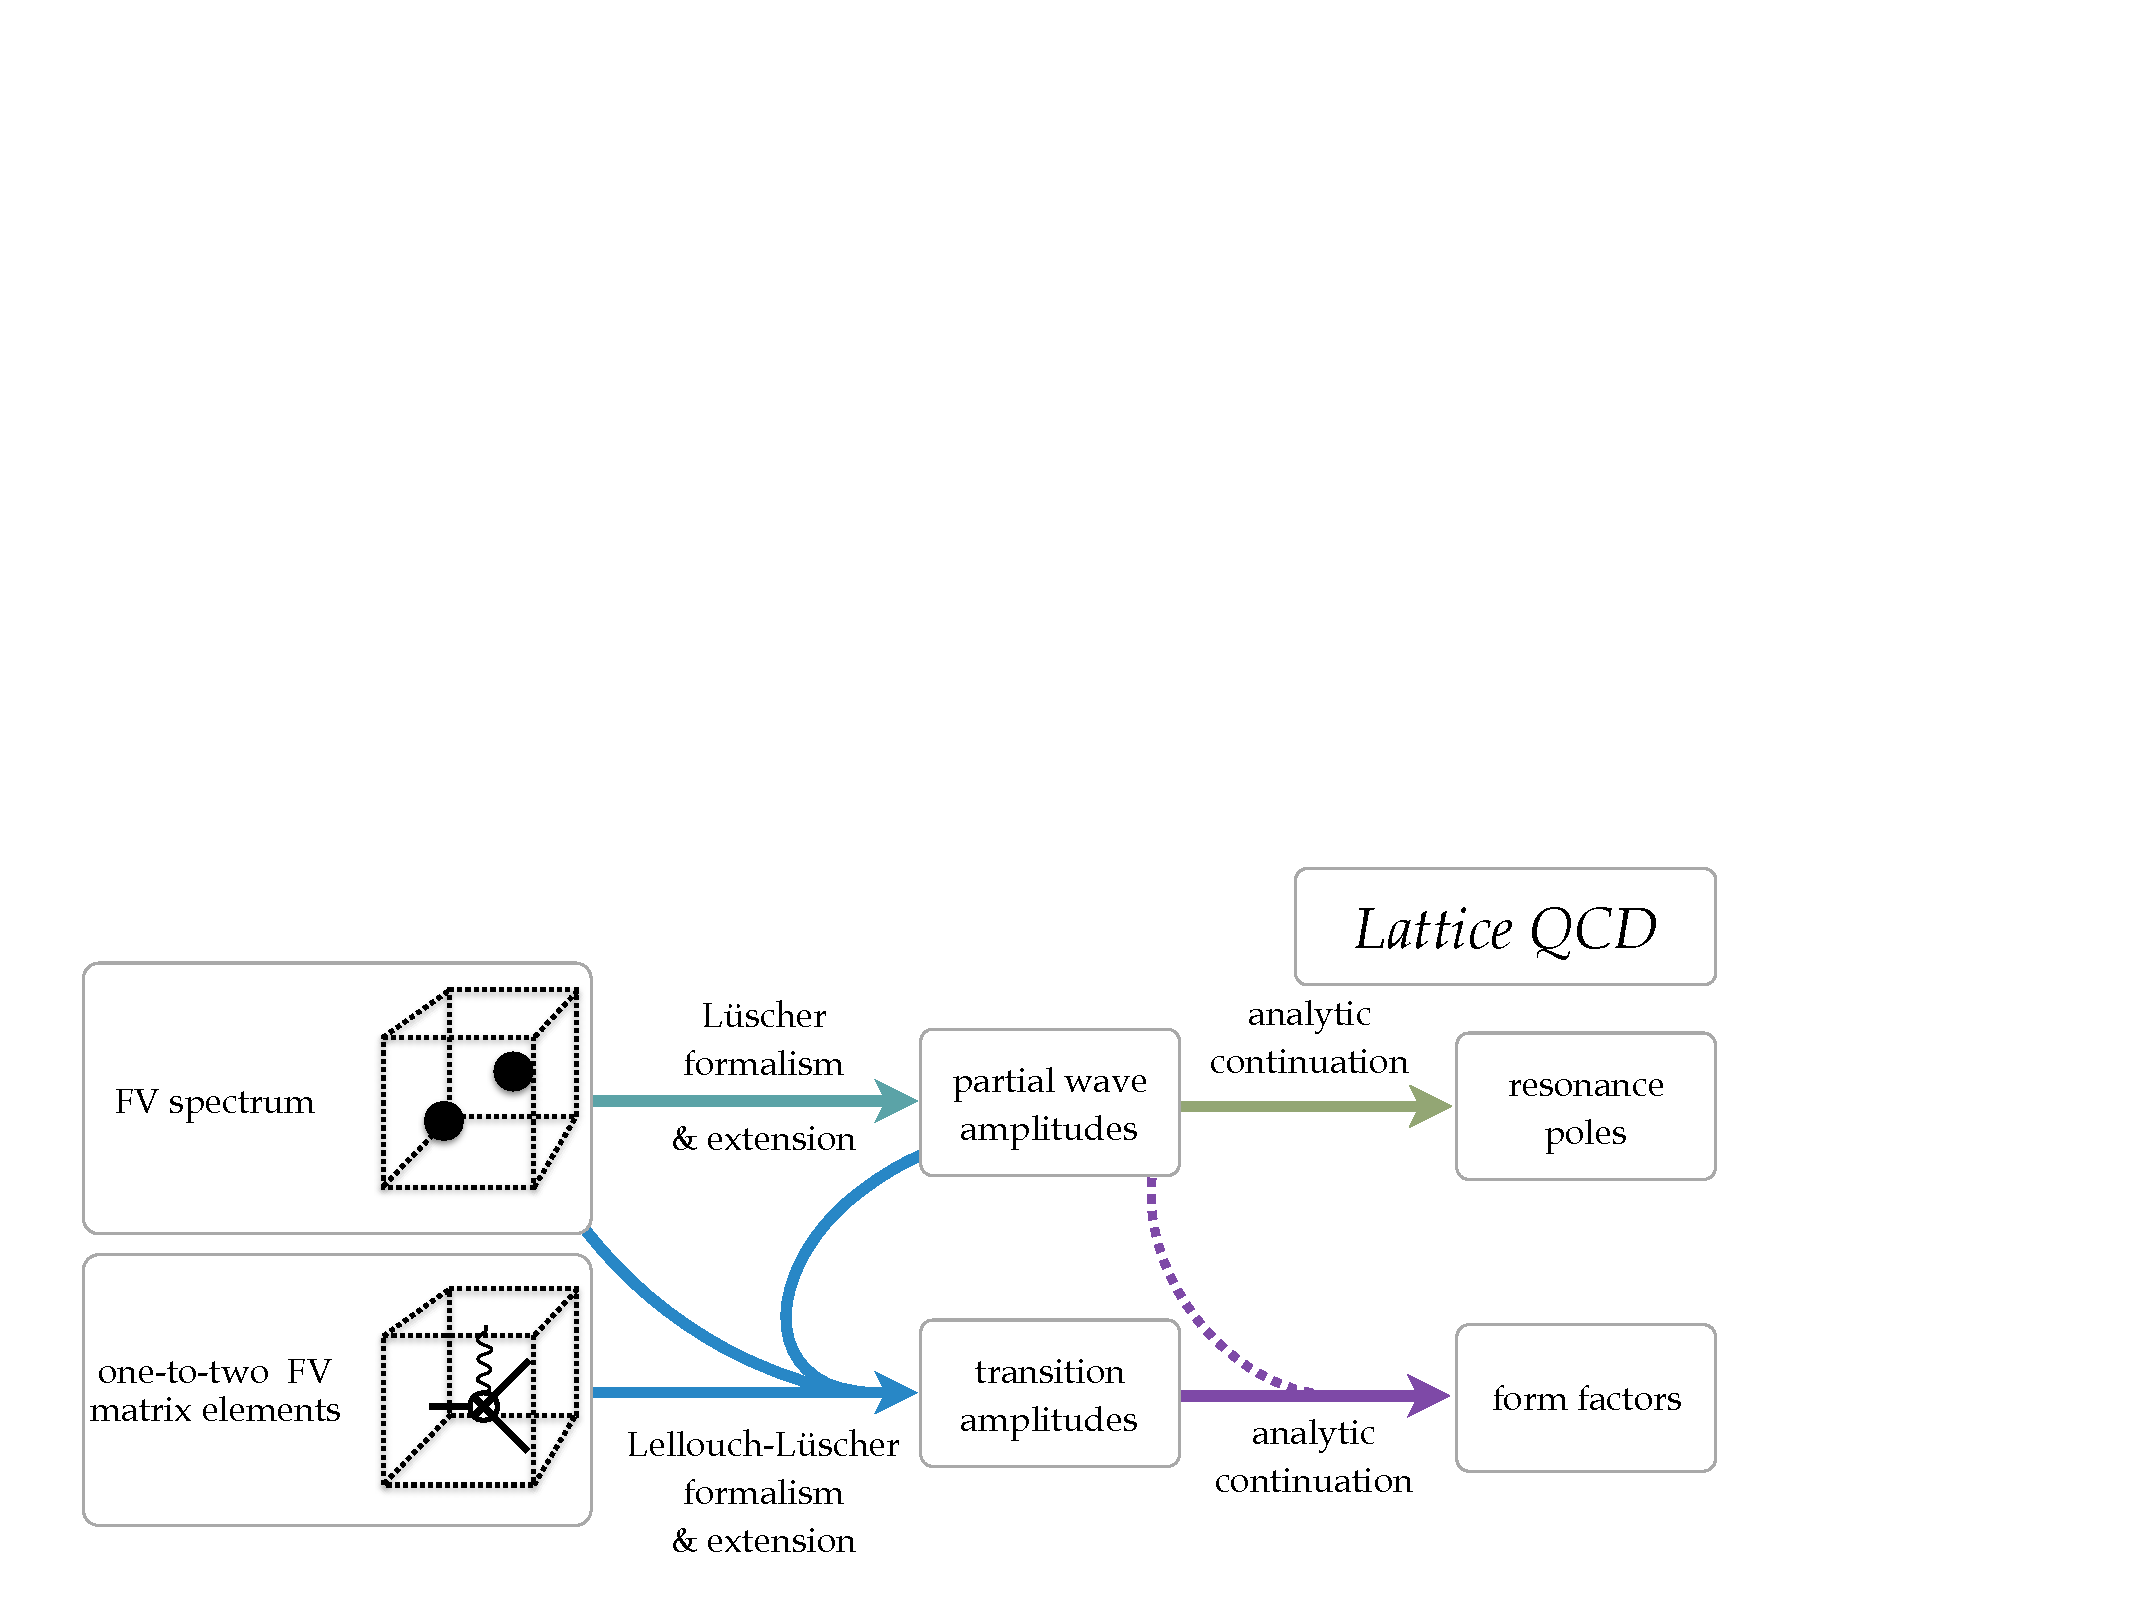
\includegraphics[scale=0.21]{LQCD_flow}
\label{fig:LQCD_flow}}
\hspace{.1cm} 
\subfigure[]{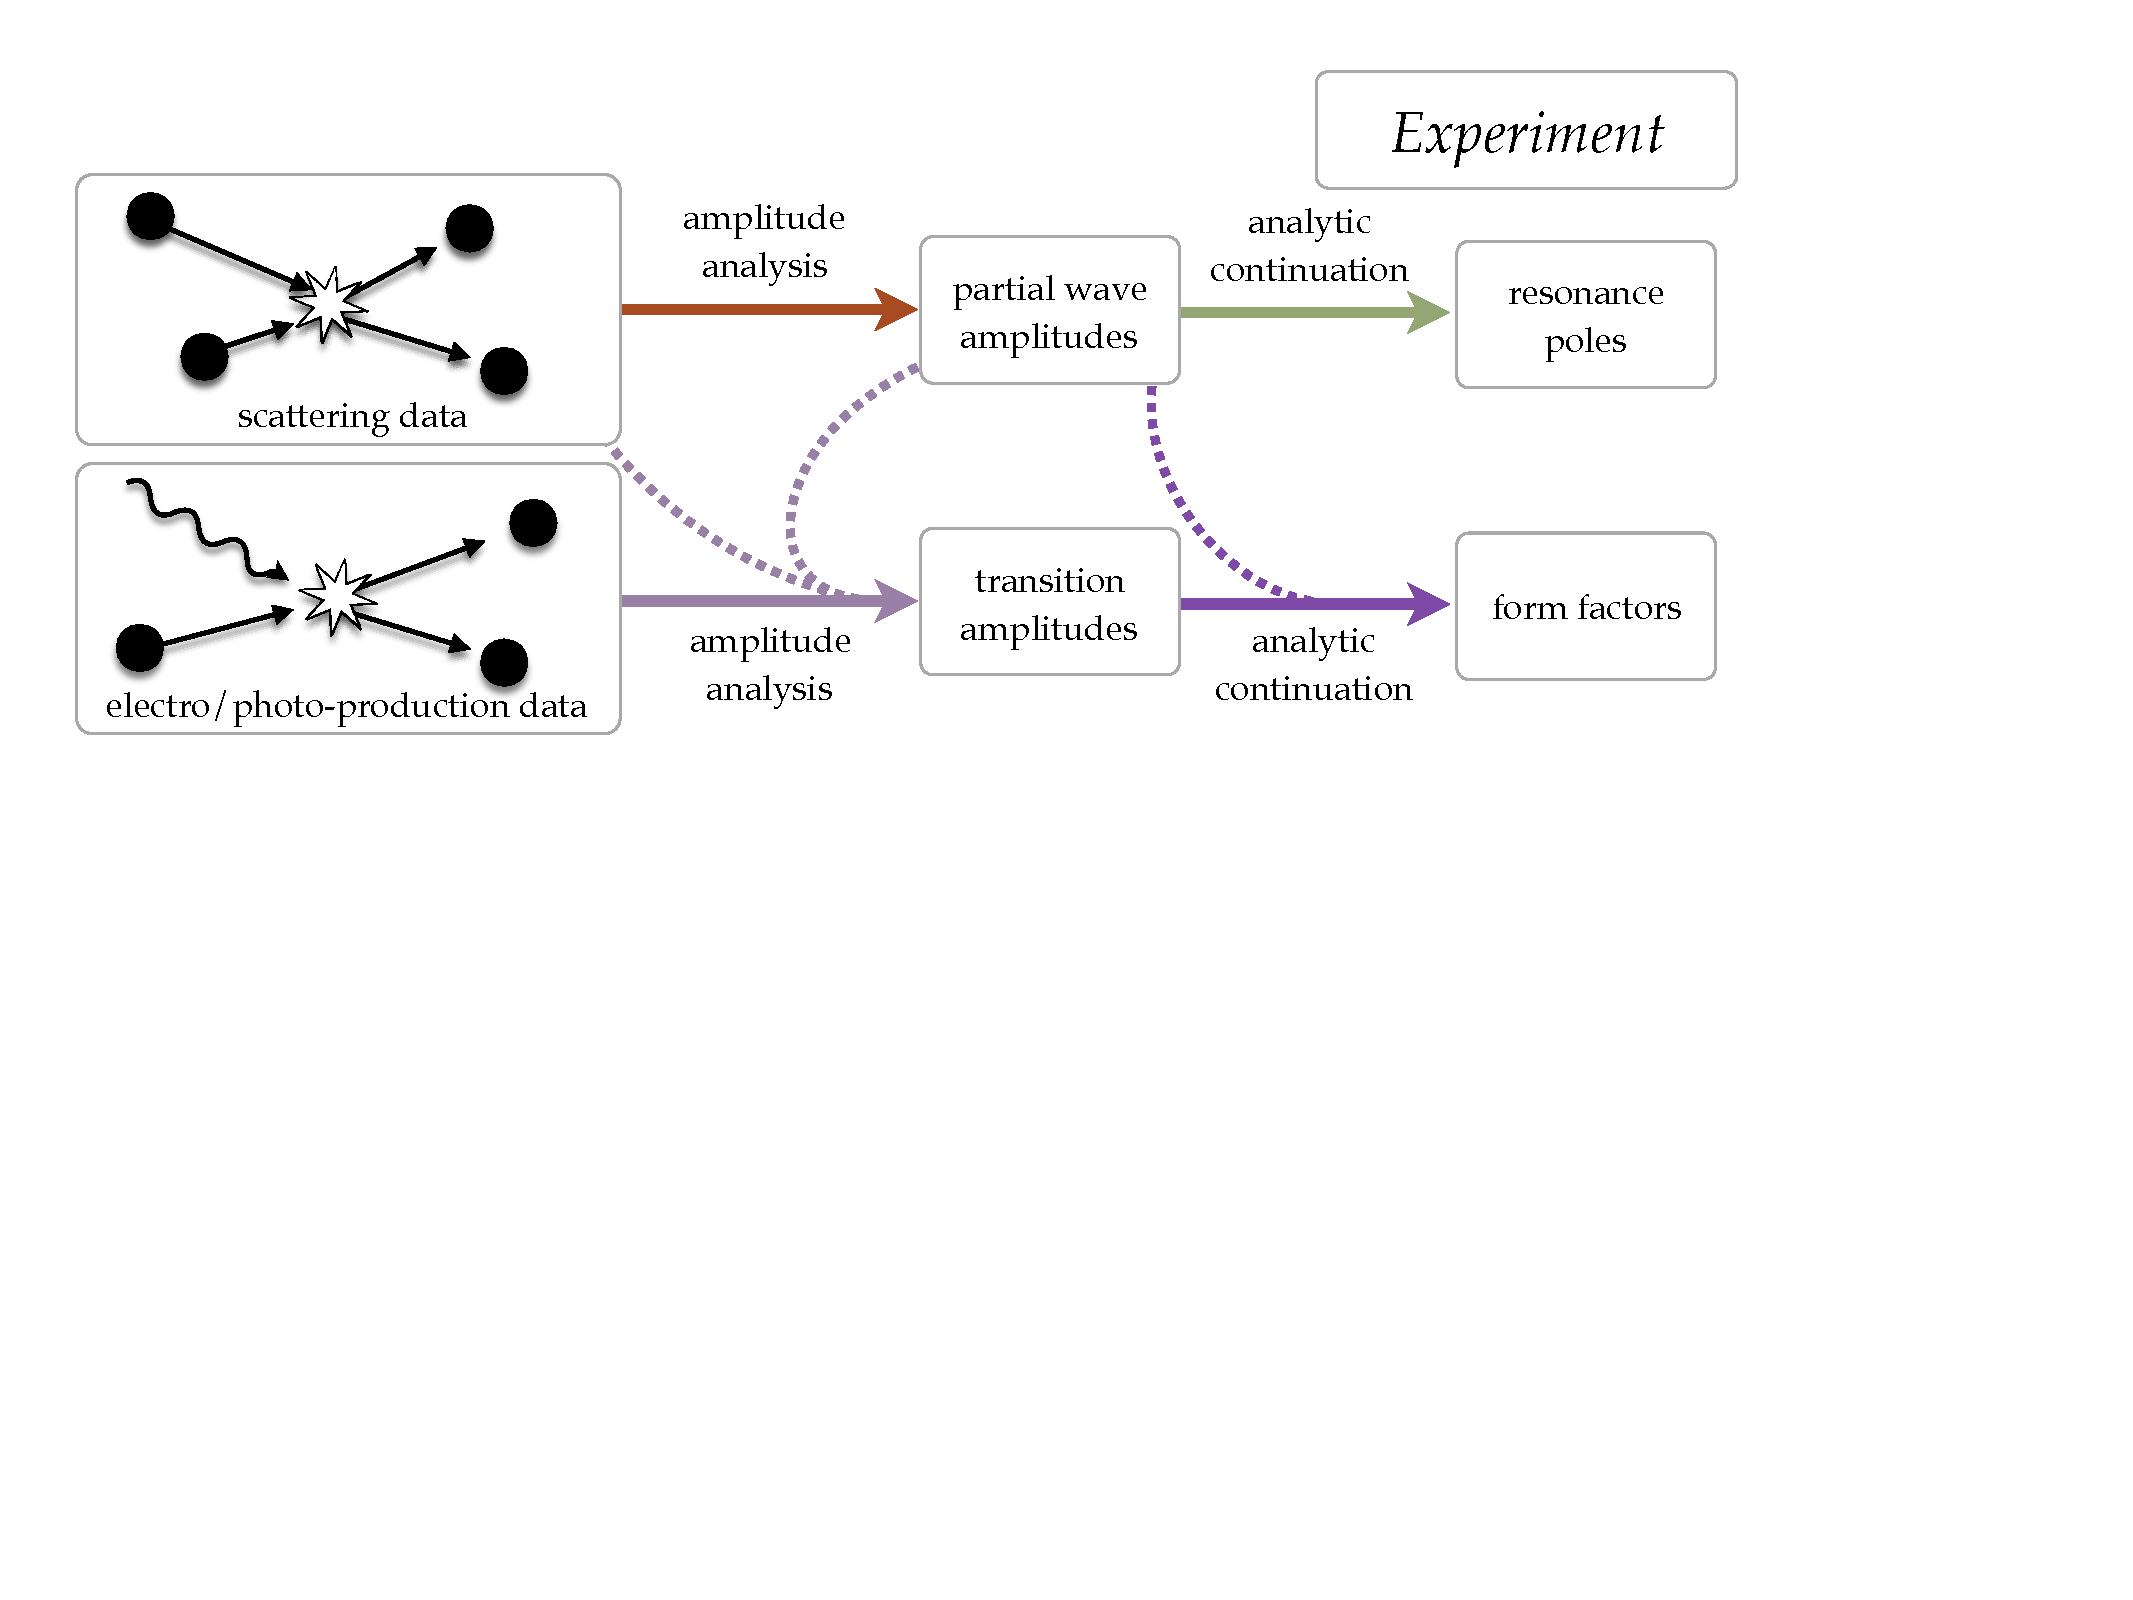
\includegraphics[scale=0.21]{Exp_flow}
\label{fig:Exp_flow}}
\caption{ (a)  (b)  This figures were first shown in Ref.~\cite{Briceno:2016cxt}.}
\label{fig:flow_charts} 
\end{figure}
%%%%%%%%%%%%%%%%
%%%%%%%%%%%%%%%%
%%%%%%%%%%%%%%%%

As will be reviewed below, the transitions amplitudes exhibit some of the same analytic structure of the scattering amplitude. In particular, the both will have the same poles in the complex place associated with resonances. From the residue of the transition amplitude one can defined \emph{form factors} of hadronic resonances. This was first suggested in Refs.~\cite{Bernard:2012bi, Agadjanov:2014kha, Briceno:2015csa}, and it was only been implemented in Ref.~\cite{Briceno:2015dca} in the determination of the $\rho\to\pi\gamma^\star$ form factor. In Sect.~\ref{sec:trans_amps}, we review the relation between the transition amplitude and the form factor for some simple examples. 

The form factors of resonances are are quantities that are fairly new to the lattice QCD community. As a step towards introducing these, we first review quantities that are customarily calculated by the lattice QCD community, namely the form factors of QCD-stable hadrons. 
%%%%%%%%%%%%%%%%%%%%%%%%%%%%%%%
%%%%%%%%%%%%%%%%%%%%%%%%%%%%%%%

\subsection{Matrix elements, decay constants, and form factors of QCD-stable particles\label{sec:ff_stable}}
Lattice QCD calculations of form factors for stable hadronic states has reached a remarkable level of sophistication. Although we cannot review all the progress made, it is worth highlighting two major developments in recent years. First, physical-point calculations are currently underway for ``\emph{simple}" observables~\cite{Abdel-Rehim:2016won, Green:2014xba, Owen:2015gva}. Second, it has been demonstrated that form factors of excited states are indeed accessible via lattice QCD~\cite{Shultz:2015pfa}. The second of these is of crucial for the determination of form factors of resonances. To understand the significance of this, we review the determination of matrix elements from lattice QCD. 

Matrix elements of external currents can be obtained from the evaluation of three-point functions. For simplicity, we begin by defining two-point functions, which are commonly use in the determination of the finite-volume spectrum. We conveniently follow the notation used in Ref.~\cite{Briceno:2015tza}. Let $B^\dagger$ and $\mathcal A$ be creation and annihilation operators, respectively.  We need not specify any details of either one of the operators, except that they must both have the quantum numbers of the states we wish to study. We can then proceed to write the standard definition of the two-point function in a finite Euclidean spacetime,
\begin{eqnarray}
C_L(x_4-y_4, \mathbf P)   \equiv \int_L \! d \mathbf x \int_L \! d \mathbf y \ e^{- i \mathbf P \cdot (\mathbf x - \mathbf y)} \Big [ \langle 0 \vert T \mathcal A(x) \mathcal B^\dagger(y) \vert 0 \rangle \Big ]_L \,,
\label{eq:two-point}
\end{eqnarray}
 where $x_4-y_4$ is the time separation between the source and sink and $\mathbf P$ is the total momentum of the system, and $T$ denotes that one must considered the time-ordered product of the operators. By inserting a complete set of finite-volume states and identifying $B^\dagger$ and $\mathcal A$ as Heisenberg operators in Euclidean spacetime, one can rewrite the two-point function as a sum over decaying exponentials in time,
 \begin{eqnarray}
\hspace{-2.2cm}
C_L(x_4-y_4, \mathbf P) & \equiv& \int_L \! d \mathbf x \int_L \! d \mathbf y \ e^{- i \mathbf P \cdot (\mathbf x - \mathbf y)} \Big [ \langle 0 \vert T \mathcal A(x) \mathcal B^\dagger(y) \vert 0 \rangle \Big ]_L \,, \nn\\
& =& \int_L \! d \mathbf x \int_L \! d \mathbf y \ e^{- i \mathbf P \cdot (\mathbf x - \mathbf y)} \sum_n \Big [ \langle 0 \vert \mathcal A(x_4, \mathbf x)  \vert E_n, \mathbf P, L \rangle \Big ]_L \Big [ \langle E_n, \mathbf P, L \vert \mathcal B^\dagger(y_4, \mathbf y) \vert 0 \rangle \Big ]_L\,, \nn\\
%& =&  \int_L \! d \mathbf x \int_L \! d \mathbf y \ \sum_n e^{- E_{n,\mathbf P,L}(x_4-y_4)}  \Big [  \langle 0 \vert  \mathcal A(0)  \vert E_n, \mathbf P, L \rangle \Big ]_L \Big [ \langle E_n, \mathbf P, L \vert \mathcal B^\dagger(0) \vert 0 \rangle \Big ]_L \,, \nn\\
& =&  L^6 \sum_n e^{- E_{n}(x_4-y_4)}   \Big [ \langle 0 \vert  \mathcal A(0)  \vert E_n, \mathbf P, L \rangle \Big ]_L \Big [ \langle E_n, \mathbf P, L \vert \mathcal B^\dagger(0) \vert 0 \rangle \Big ]_L \,.
\label{eq:completeset}
\end{eqnarray}
This equation requires some explanation. $E_{n}$ denotes the energy of the $nth$ finite-volume eigenstate. Although obvious from the second equality, it is worth emphasizing that we have defined finite-volume states to be dimensionless and normalized to unity, $\langle E_n, \mathbf P_f, L \vert E_{n'}, \mathbf P_i, L \rangle = \delta_{n,n'}\delta_{\mathbf P_f, \mathbf P_i} \,$. This is the most natural prescription for finite-volume states, given the fact that there is no notion of asymptotic states, and as a result one cannot in general identify states by the number of particles present. This can be contrasted to the normalization of the infinite volume state of a single particle with mass $m$,
\begin{equation}
\langle  P_f  \vert   P_i \rangle = 2 \omega_{f} (2 \pi)^3 \delta^3(\mathbf P_f- \mathbf P_i) \,,
\end{equation}
where $ P_f^0= \omega_{f} = \sqrt{\mathbf P_f ^2 + m^2}$. The brackets above, $\Big [  ~\Big ]_L$, emphasize that the matrix elements operators are evaluated in a finite volume $V=L^3$. 

One can observe that any given operator has overlap with an infinite tower of states. By waiting for sufficiently long times, the correlation function will be dominated by the ground state. {\raul Disentangling the large tower of state is a formidable task, that we will touch on...} 

For states that lie well below the $N(\geq2)$-body thresholds, one can readily show that the  finite-volume overlap appearing in the two-point function above are proportional to their infinite volume counterpart. For example, let $B^\dagger$ have the quantum number of the $\pi$, and let $\mathcal A\to \mathcal A_\mu=\bar{\psi}\gamma_\mu\gamma_5\psi$ be the axial vector current. In the infinite volume, Lorentz invariance and parity conservation dictates that
\begin{eqnarray}
\label{eq:fpi}
\langle 0 \vert  \mathcal A_\mu(0)  \vert \pi, P \rangle 
=P_\mu f_\pi,
\end{eqnarray}
where $f_\pi$ is the $\pi$ decay constant, and it  `\emph{parametrizes our ignorance}'. Given that the $\pi$ is a QCD stable particle, one can show that for sufficiently large volumes satisfying $m_\pi L \gg 1$, the finite-volume state corresponding to the $\pi$ is exponentially close to its infinite-volume counterpart~\cite{Luscher:1985dn}. In fact, had we used an alternative normalization for the finite volume states, we would arrive at an identical expression for the finite-volume matrix element of the axial current. One can show, 
\begin{eqnarray}
\label{eq:fpi_L}
\big[\langle 0 \vert  \mathcal A_\mu(0)  \vert \pi, P \rangle\big] _L
=\frac{P_\mu f_\pi}{\sqrt{2\omega_\pi L^3}},
\end{eqnarray}
where the factor appearing in the denominator corrects for the finite-volume state normalization. When the energy of the finite-volume state lies above a $N(\geq2)$-body threshold, the interpretation of the finite-volume overlap factor is more subtle. In Sect.~\ref{sec:LL_formalism} we discuss the presently available formalism for studying these when the finite-volume state couples only to two-particle states. 


To obtain, for example, the elastic form factor of state, we must then consider the evaluation of three-point functions. These are similar to the two-point function defined in Eq.~\ref{eq:two-point}, except between the source and sink operator one must insert an external current $\mathcal{J}$, 
\begin{eqnarray}
\hspace{-2.2cm}
C_L^{2\rightarrow 2}(x_{f,4}-y_{4},y_{4}-x_{i,4}, \mathbf P_i, \mathbf P_f) &&\nn\\
&&\hspace{-4.5cm}\equiv \int_L \! d \mathbf x_f~ \! d \mathbf x_i ~ \! d \mathbf y
 \ e^{- i \mathbf  P_f \cdot (\mathbf x_f - \mathbf y)} 
  \ e^{- i \mathbf  P_i \cdot (\mathbf y - \mathbf x_i)} 
  \times  \Big [ \langle 0 \vert T 
  \mathcal A(x_f) 
  {\mathcal{J}}(y)\mathcal B^\dagger(x_i) \vert 0 \rangle \Big ]_L \,.   \label{eq:three-point_func}
  \end{eqnarray}
 Unlike in the case of the two-point functions, the operators $  \mathcal A$ and $\mathcal B$ need not have the same quantum numbers. Just like before, it is convenient to introduce complete sets of states, to rewrite this correlation function as a linear combination of exponentials,
\begin{eqnarray}
\hspace{-2.2cm}
C_L^{2\rightarrow 2}(x_{f,4}-y_4,y_4-x_{i,4}, \mathbf P_i, \mathbf P_f) &&
=  L^9 \sum_{n_i,n_f} 
  e^{- E_{n_f}(x_{f,4}-y_4)}
  e^{- E_{n_i}(y_4-x_{i,4})}\nn\\
 &&\hspace{-5.5cm}
 \times
\Big [ \langle 0 \vert  \mathcal A(0)  \vert E_{n_f}, \mathbf P_f, L \rangle \Big ]_L 
\Big [ \langle E_{n_f}, \mathbf P_f, L \vert  \mathcal J(0)  \vert E_{n_i}, \mathbf P_i, L \rangle \Big ]_L 
\Big [ \langle E_{n_i}, \mathbf P_i, L \vert \mathcal B^\dagger(0) \vert 0 \rangle \Big ]_L.
\label{eq:3pt_completeset}
\end{eqnarray}
In general, the physical meaning of $\Big [ \langle E_{n_f}, \mathbf P_f, L \vert  \mathcal J(0)  \vert E_{n_i}, \mathbf P_i, L \rangle \Big ]_L$ strongly depends on the nature of the initial and final state. In Sec.~\ref{sec:LL_formalism}, we discuss the interpretation of this matrix element when the initial state couples to a two-particle states and the final state couples to a one-particle state. In Sec.~\ref{sec:2body_mat} we explain the interpretation of this when both then initial and final states couple to two-particle states. 

First, we restrict our attention to the scenario where both the initial and final correspond to the $\pi$, and the external is the electromagnetic current $\mathcal J^\mu=(2\bar{u}\gamma^\mu u-\bar{d}\gamma^\mu d-\bar{s}\gamma^\mu s)/{3}$. One can show that the infinite-volume matrix element must have the form,
\begin{eqnarray}
\label{eq:pi_ff}
\langle  \pi, P_f \vert  \mathcal J^\mu(0)  \vert \pi, P_i \rangle 
=(P_i+P_f)^\mu F_\pi(Q^2),
\end{eqnarray}
where $F_\pi(Q^2)$ is the elastic $\pi$ electromagnetic form factor and $Q^2=-(P_i-P_f)^2$ is commonly referred to as the virtuality of the external photon. When $Q^2=0$ the external photon corresponds to a physical one and the form factor satisfies $F_\pi(0)=1$. We have used symmetry arguments to arrive at Eq.~\ref{eq:pi_ff}, but such arguments are not sufficient to constrain the form factor. 

Once again, the relationship between the lattice QCD matrix elements and the form factor is only complicated by the normalization of the finite-volume states, 
\begin{eqnarray}
\label{eq:pi_ff_L}
\big[
\langle  \pi, P_f \vert  \mathcal J^\mu(0)  \vert \pi, P_i \rangle\big] _L
=\frac{(P_i+P_f)^\mu F_\pi(Q^2),}{\sqrt{(2\omega_iL^3 )(2\omega_f L^3)}}.
\end{eqnarray}
This is exact up to corrections of the form $\mathcal{O}(e^{-m_\pi L})$. By utilizing volumes satisfying $m_\pi L\geq 1$, one can directly determine infinite-volume form factors of stables hadronic states. This is what has allowed for the determination of, for example, the calculations of the $\pi$ and nucleon form factors \cite{Green:2015wqa, Shultz:2015pfa}. Said calculations can be computationally taxing and at times they require the development of cutting edge algorithms, for example when they require the determination of disconnected quark-loop diagrams~\cite{Green:2015wqa, Gambhir:2016uwp}. Yet, it is fair to say these are, otherwise, conceptually straightforward observables. On the other hand, the form factor of a resonance is not at all a familiar observables. In fact, to this day, there has been a single calculation of a resonance form factor from lattice QCD~\cite{Briceno:2015dca, Briceno:2016kkp}. Therefore, before proceeding to discuss how such form factors can accessed from lattice QCD, we will begin by defining said observables. 





%%%%%%%%%%%%%%%%%%%%%%%%%%%%%%%
%%%%%%%%%%%%%%%%%%%%%%%%%%%%%%%
\subsection{Transition amplitudes and form factors of resonance\label{sec:trans_amps}}
As has already been discussed, resonance are not asymptotic states,  


\cite{Bernard:2012bi, Agadjanov:2014kha, Agadjanov:2016qdz}

\cite{Gegelia:2009py, Hoja:2010fm, Albaladejo:2012te}

%%%%%%%%%%%%%%%%%%%%%%%%%%%%%%%
%%%%%%%%%%%%%%%%%%%%%%%%%%%%%%%
\subsection{Lellouch-L\"uscher's formalism and its generalizations~\label{sec:LL_formalism}}
Talk about $1\to2$ and $0\to2$ transitions.
%%%%%%%%%%%%%%%%%%%%%%%%%%%%%%%
%%%%%%%%%%%%%%%%%%%%%%%%%%%%%%%
\subsection{Finite volume matrix elements of two-particle states~\label{sec:2body_mat}}
Naively, one would expected an LL factor for the initial and final state.
%%%%%%%%%%%%%%%%%%%%%%%%%%%%%%%
%%%%%%%%%%%%%%%%%%%%%%%%%%%%%%%
\subsection{Perturbative results~\label{sec:perturbative_results}}
Similarly as was reviewed in Sect.~\ref{}, one can find a relationship between finite volume matrix elements and infinite volume low-energy coefficients. This was done in Ref.~[] systems composed of scalar mesons with weakly repulsive interactions. This result has the advantage of being relatively simple to apply in the analysis of matrix elements. 
%%%%%%%%%%%%%%%%%%%%%%%%%%%%%%%
%%%%%%%%%%%%%%%%%%%%%%%%%%%%%%%
\subsection{Background field methods~\label{sec:background_field}}
To this day, this has not been successfully implemented in the study of matrix elements of scattering states. 

\cite{Davoudi:2015cba, Davoudi:2015zda}
%%%%%%%%%%%%%%%%%%%%%%%%%%%%%%%
%%%%%%%%%%%%%%%%%%%%%%%%%%%%%%%
\subsection{Optical potential in a finite-volume~\label{sec:optical_potential}}



%%%%%%%%%%%%%%%%%%%%%%%%%%%%%%%
%%%%%%%%%%%%%%%%%%%%%%%%%%%%%%%

%%%%%%%%%%%%%%%%%%%%%%%%%%%%%%%
%%%%%%%%%%%%%%%%%%%%%%%%%%%%%%%
\subsection{Scattering from lattice QCD+QED calculations~\label{sec:trans_amps}}
%%%%%%%%%%%%%%%%%%%%%%%%%%%%%%%
%%%%%%%%%%%%%%%%%%%%%%%%%%%%%%%
\subsection{Long range effects~\label{sec:trans_amps}}
draw long range effects contributing to gamma+gamma scatterging

\cite{Briceno:2015dca}


%%%%%%%%%%%%%%%%%%%%%%%%%%%%%%%
%%%%%%%%%%%%%%%%%%%%%%%%%%%%%%%

\begin{table}
  \begin{tabularx}{\textwidth}{c|c|c|c|c}
    \hline\hline
~& Non-pert./pert.& PW mixing& Multichannels&Universal\\
\hline\hline
\multirow{3}{*}{$1\to2$/$0\to2$~\cite{Briceno:2015csa}} &&&&  \\
&Non-pert. &\gcheck&\gcheck &\gcheck  \\
&&&&  \\
\hline
\multirow{3}{*}{$2\to2$~\cite{Briceno:2015tza}}&&&&  \\
&Non-pert. &\gcheck&\gcheck &\gcheck  \\
&&&&  \\
\hline
\multirow{3}{*}{$N\to N(N>2)$~\cite{Detmold:2014fpa}}&&&&  \\
&Pert. &\xmark&\xmark &\xmark  \\
&&&&  \\
\hline
\multirow{3}{*}{Background field~\cite{Detmold:2004qn}}&&&&  \\
&Non-pert. &\xmark&\xmark &\xmark  \\
&&&&  \\
   \hline
\multirow{3}{*}{QED+QCD scat.~\cite{Beane:2014qha}}&&&&  \\
&Pert. &\xmark&\xmark &\xmark  \\
&&&&  \\
   \hline
\multirow{3}{*}{long range effects~\cite{Christ:2015pwa}}&&&&  \\
&Non-Pert. &\xmark&\xmark &\xmark  \\
&&&&  \\
   \hline
  \end{tabularx}
    \caption{.......?}
\end{table}
%%%%%%%%%%%%%%%%%%%%%%%%%%%%%%%
%%%%%%%%%%%%%%%%%%%%%%%%%%%%%%%


\section*{References}

%\bibliographystyle{numeric-comp}
\bibliographystyle{unsrt.bst}
\bibliography{bibi}

%%%%%%%%%%%%%%%%%%%%%%%%%%%%%%%%%%%%%%%%%%%%%%%%%%%%%%%%%%%%

\end{document}
